\documentclass[recuosum=1.5cm]{iftex2024}

\usepackage{numprint}
\npthousandsep{.}
\npdecimalsign{,}

% \DeclareUnicodeCharacter{0301}{XXXXXXXXXXXXXXXXXXXXXXXXXXXX}
\usepackage[backend=biber]{biblatex}

\usepackage{xcolor}
\usepackage{minted}
\usepackage{dirtree}
\usepackage{longtable}
\usepackage{booktabs}
\renewcommand{\arraystretch}{1.2}  % mais espaço entre linhas
\usepackage{makecell}


\usemintedstyle{borland}
\definecolor{LightGray}{gray}{0.95}

\usepackage{caption}
\usepackage{etoolbox}

% Contador para códigos
\newcounter{codigo}[chapter]
\renewcommand{\thecodigo}{\thechapter.\arabic{codigo}}

% Comando para título e label do código
\newcommand{\codigo}[2]{%
	\refstepcounter{codigo}%
	\noindent\captionof*{table}{\textnormal{Código~\thecodigo{} -- #1}}\label{#2}%
}

\addbibresource{referencias.bib}
\titulo{Análise e integração de dados do mercado financeiro brasileiro disponibilizados pela B3 e CVM}
\autor{Vinícius Tadeu Andrade Costa}
\local{Bambuí -- MG}
\data{2025-01-18}

\campus{\textit{Campus} Bambuí}
\curso{Bacharelado}{Engenharia de Computação}
\titulacao{Bacharel}

\orientador[M]{Marcos Roberto Ribeiro}
% \coorientador{Nome da Coorientador}
% \instituicaocoorientador{Instituição do Coorientador}
% \membrobanca{Fulano de Tal}{Instituição do Fulano de Tal}
% \membrobanca{Ciclano de Tal}{Instituição do Ciclano de Tal}
% \fichacatalografica{ficha.pdf}
% \assinaturas{assinaturas.pdf}

\dedicatoria{Dedico este trabalho à minha esposa e filhos, incentivadores e fontes inesgotáveis de apoio, amor e compreensão.}

\agradecimentos{Agradeço a toda à minha família, esposa, filhos, pais e minha irmã, por acreditarem em mim e pelo incentivo constante na realização deste trabalho.

Agradeço à minha orientadora, ao meu coorientador e a todos que contribuíram de alguma forma para a realização deste trabalho.}

\epigrafe{A tarefa mais importante de uma pessoa que vem ao mundo é criar algo.}{Paulo Freire}

\resumo{Este trabalho é um modelo em {\latex} utilizando a classe \iftex.
Tal classe foi desenvolvida com base no manual de normalização de trabalhos acadêmicos do IFMG e nas normas relacionadas da Associação Brasileira de Normas Técnicas.
Este modelo apresenta uma estrutura básica com exemplos de elementos pré e pós-textuais.
Maiores informações sobre como utilizar a classe podem ser encontradas no manual da classe \iftex.}
\palavraschave{\iftex. Modelo. IFMG. \latex.}

\abstract{This work is a template in {\LaTeX} using the \iftex class.
This class was developed based on the academic work standardization manual of IFMG and the related norms of the Brazilian Association of Technical Standards.
This template presents a basic structure with examples of pre and post-textual elements.
Further information on how to use the class can be found in the \iftex class manual.}
\keywords{\iftex. Template. IFMG. \latex.}

\listafiguras
\listaquadros
\listatabelas

\listasiglas{%
 \begin{itemize}[]
  \item[IFMG] -- Instituto Federal de Educação, Ciência e Tecnologia de Minas Gerais
  \item[TCC] -- Trabalho de conclusão de curso
  \item[B3] -- Brasil, Bolsa e Balcão
  \item[CVM] -- Comissão de Valores Mobiliários
  \item[DFP] -- Demonstrações Financeiras Padronizadas
  \item[ITR] -- Formulário de Informações Trimestrais
  \item[IPE] -- Periódicos e Eventuais
  \item[FRE] -- Formulário de Referência
 \end{itemize}
}

\listasimbolos{%
 \begin{itemize}[]
   \item[$\mathbb{X}$] -- Variável X
   \item[$\mathsf{I\!R}$] -- Conjunto dos números reais
 \end{itemize}
}

\begin{document}

\maketitle

\chapter{INTRODUÇÃO}

 \index{INTRODUÇÃO}
Este capítulo contextualiza o trabalho e delineia seus objetivos. A Seção~\ref{sec:justificativa} apresenta as motivações e os desafios que justificam a integração automatizada dos dados financeiros públicos. Na Seção~\ref{sec:objetivos}, são expostos o objetivo geral e as metas específicas desta pesquisa. Por fim, a Seção~\ref{sec:resultados} discute os resultados esperados com a solução proposta.

O mercado financeiro brasileiro tem passado por transformações significativas impulsionadas pelo avanço tecnológico e pela crescente demanda por soluções que automatizem a integração e a análise de dados \cite{dantas:2020:comportamento}. Esse movimento reflete a busca constante por maior eficiência e acessibilidade nas informações financeiras, fundamentais para investidores e analistas que utilizam a análise fundamentalista como base para a tomada de decisões.

O crescimento desse interesse pode ser observado no relatório anual de 2023 da Brasil, Bolsa e Balcão (B3), que apontou um aumento de aproximadamente 15\% no número de investidores em comparação com 2022 \cite{b3:2023:relatorio}. Esse cenário reforça a necessidade de garantir o acesso simplificado e estruturado às informações financeiras das empresas, promovendo maior eficiência nas análises e decisões de mercado.

No Brasil, dois órgãos desempenham papéis centrais na disponibilização de dados do mercado de capitais: a B3 e a Comissão de Valores Mobiliários (CVM). A B3, fundada em 1890 e sediada em São Paulo, é a única bolsa de valores do país e fornece dados sobre o histórico de negociações de ativos \cite{b3:2023:investidores}. 

Já a CVM, criada em 1976, é a entidade responsável por regulamentar e supervisionar o mercado de capitais brasileiro, disponibilizando publicamente uma ampla gama de informações contábeis e financeiras das empresas listadas na bolsa \cite{cvm:2009:informacao}. Essas informações são essenciais para investidores que utilizam a análise fundamentalista, metodologia que avalia a saúde financeira e o desempenho das empresas com base em seus demonstrativos financeiros e outros indicadores econômicos.

Embora a CVM disponibilize esses dados publicamente, seu formato dificulte a manipulação por usuários sem conhecimento técnico avançado. Muitos estão em arquivos complexos que exigem processamento adicional, criando um obstáculo para investidores e analistas que necessitam de informações ágeis e acessíveis. Essa barreira técnica restringe o acesso à informação e limita a capacidade analítica de boa parte do mercado.

A necessidade de soluções mais acessíveis já foi abordada por estudos acadêmicos. \cite{deAraujo:2021:modeloDados} propõem um modelo de dados flexível para análise fundamentalista moderna, estruturando balanço patrimonial, demonstração de resultados e fluxo de caixa em um banco de dados não relacional (MongoDB). Esse tipo de abordagem reforça a importância de alternativas que simplifiquem o acesso e a análise dos dados financeiros.


Diante desse contexto, este trabalho propõe o desenvolvimento de um sistema automatizado para a integração e análise dos dados fornecidos pela CVM, facilitando seu acesso e processamento. A solução busca oferecer uma ferramenta capaz de extrair e estruturar essas informações de forma eficiente, contribuindo para a análise fundamentalista e auxiliando na tomada de decisões. Além disso, pretende otimizar o processo de análise, tornando-o mais acessível e organizado para investidores, analistas e pesquisadores. Com essa abordagem, espera-se reduzir a complexidade no manuseio dos dados e aprimorar a compreensão do mercado.

\section{Justificativa}\label{sec:justificativa}
A B3 apresentou um crescimento significativo no volume de negócios e de capital movimentado ao longo dos anos. Em 2023, o volume total negociado na B3 alcançou R\$ 7,2 trilhões, representando um aumento de 12,6\% em relação a 2022 \cite{b3:2023:investidores}. Além disso, o montante total de dinheiro movimentado na B3 em 2023 foi de R\$ 2,4 trilhões, um aumento de 15,5\% em relação ao ano anterior \cite{b3:2023:investidores}.

Embora os dados da B3 não estejam diretamente presentes neste trabalho, seu contexto é fundamental, uma vez que ela representa o principal ambiente de negociação de ativos no Brasil. As informações que embasam os negócios realizados na B3, especialmente aquelas relacionadas às demonstrações financeiras e dados cadastrais das empresas listadas, estão disponíveis na CVM. Dessa forma, a integração dos dados da CVM serve como uma base fundamental para análises que indiretamente impactam o entendimento do mercado da B3.

Atualmente, as informações da CVM estão disponíveis em formatos específicos, fragmentados e sem integração adequada, o que dificulta o acesso e a análise automatizada dos dados. Até o momento, não foram encontrados trabalhos que promovam essa integração de forma estruturada e com disponibilização pública.

A proposta de integrar os dados da CVM visa criar uma base de dados unificada e acessível, que sirva como suporte para futuros trabalhos acadêmicos e aplicações práticas em algoritmos de análise de mercado financeiro. Com isso, espera-se facilitar o desenvolvimento de estudos e ferramentas que contribuam para uma melhor compreensão do mercado de capitais brasileiro \cite{lindman:2020:integration}

\section{Objetivos}\label{sec:objetivos}

Este estudo tem como objetivo principal o desenvolvimento de um sistema automatizado capaz de integrar e facilitar o acesso aos dados financeiros disponibilizados publicamente pela CVM. A proposta busca contribuir com a análise fundamentalista e apoiar o processo de tomada de decisão por parte de investidores, pesquisadores e demais interessados no mercado financeiro.

Para atingir esse objetivo, são estabelecidas as seguintes metas específicas:

\begin{itemize} 
	\item analisar a estrutura dos dados públicos fornecidos pela CVM, identificando suas fontes, formatos e padrões; 
	\item propor uma modelagem lógica que permita a integração eficiente e automatizada desses dados; 
	\item projetar e implementar um sistema que realize a extração, o processamento e a disponibilização dos dados de forma acessível e estruturada. 
\end{itemize}


\section{Resultados Esperados}\label{sec:resultados}

Espera-se que a ferramenta desenvolvida neste trabalho integre de forma eficiente os dados financeiros públicos disponibilizados pela CVM, permitindo a criação de uma base de dados unificada, estruturada e acessível.

Essa base será construída com foco em um recorte histórico que contemple, no mínimo, o período a partir de 2019, o que proporcionará maior profundidade nas análises e permitirá identificar padrões e variações ao longo do tempo. Tal histórico é essencial para estudos mais robustos e comparativos dentro do contexto da análise fundamentalista.

Embora os dados da B3 não sejam utilizados diretamente neste trabalho, o sistema proposto pode contribuir indiretamente para análises relacionadas à bolsa de valores, uma vez que as informações integradas da CVM servem como base para decisões tomadas por investidores e instituições que atuam no ambiente da B3.

A disponibilização pública dessa base de dados tem o potencial de promover maior transparência, acessibilidade e democratização das informações financeiras no Brasil, beneficiando pesquisadores, investidores e demais interessados no mercado de capitais.


\chapter{FUNDAMENTOS TEÓRICOS}

Este capítulo apresenta os fundamentos teóricos que sustentam o desenvolvimento deste trabalho, bem como os principais estudos e iniciativas relacionadas ao tema. A Seção \ref{sec:mercado-financeiro} aborda o mercado financeiro brasileiro, com ênfase na atuação da CVM e sua função reguladora. A Seção \ref{sec:analises} discute as diferentes abordagens de análise para investimentos, com foco na análise fundamentalista. A Seção \ref{sec:computacional} descreve a modelagem dos dados e os processos de integração utilizados no projeto. Por fim, a Seção \ref{sec:estado-arte} apresenta trabalhos acadêmicos e iniciativas similares à proposta deste estudo, destacando seus principais diferenciais.

\section{Mercado financeiro} \label{sec:mercado-financeiro} % OK

O mercado financeiro é um sistema que engloba uma variedade de instituições, instrumentos e atividades relacionadas à gestão de recursos financeiros. Ele abrange diferentes segmentos, incluindo o mercado de capitais, o mercado monetário, o mercado cambial e o mercado de derivativos. O principal propósito do mercado financeiro é facilitar a alocação eficiente de recursos entre poupadores e investidores, fornecendo oportunidades de investimento e financiamento para empresas, governos e indivíduos \cite{teixeira:2019:mercado, damodaran:2012:investimentos}.

No Brasil, o mercado financeiro é composto pelos segmentos de mercado de capitais, mercado monetário, mercado de crédito, mercado de câmbio e mercado de derivativos. O mercado de capitais envolve a negociação de ações, debêntures e outros ativos mobiliários. Esse segmento é fundamental para o financiamento das empresas, permitindo que elas captem recursos por meio da emissão de títulos negociáveis no mercado financeiro \cite{reis:2021:negociacao}.

O mercado monetário é o espaço onde ocorrem operações de curto prazo entre instituições financeiras e o Banco Central. Essas operações têm como objetivo controlar a liquidez da economia e a taxa de juros, garantindo o equilíbrio do sistema financeiro \cite{deSouzaFigueiredo:2021:mercado}.

O mercado de crédito destina-se ao financiamento de empresas e pessoas físicas por meio de empréstimos e financiamentos bancários. Esse segmento é essencial para a dinamização da economia, permitindo investimentos e consumo a partir da concessão de crédito.

O mercado de câmbio é responsável pelas transações de compra e venda de moedas estrangeiras. Sua função principal é viabilizar o comércio internacional, investimentos estrangeiros e a gestão de reservas cambiais \cite{gois:2019:efeito}.

O mercado de derivativos compreende a negociação de contratos futuros, opções e \textit{swaps}, instrumentos utilizados para a gestão de riscos financeiros. Esse segmento permite que investidores e empresas se protejam contra variações adversas nos preços de ativos e taxas de juros \cite{figueiredo:2023:capacidade}.

Dentro do mercado financeiro, as ações representam uma das principais modalidades de investimento. Uma ação é uma fração do capital social de uma empresa, conferindo ao seu detentor a propriedade de uma parcela da empresa emissora. Ao adquirir ações, o investidor se torna um sócio da empresa e pode ter direito a participação nos lucros distribuídos e, em alguns casos, a voto nas assembleias de acionistas \cite{reis:2021:negociacao, gomes:2007:bolsa}.

A negociação de ações ocorre principalmente em bolsas de valores, como a B3 no Brasil, onde investidores podem comprar e vender ativos. O preço das ações é determinado pela oferta e demanda, ou seja, pela interação entre compradores e vendedores no mercado \cite{santander:2024:pregao}. Além disso, diversos fatores influenciam a valorização ou desvalorização dos papéis, como os resultados financeiros das empresas, a conjuntura econômica e eventos geopolíticos \cite{damodaran:2012:investimentos, attie:2013:bolsa}.

Duas instituições fundamentais nesse ecossistema são a B3 e a CVM. A B3 atua como principal plataforma de negociação de ativos financeiros, enquanto a CVM desempenha um papel regulador crucial, garantindo transparência e equidade no mercado de capitais \cite{cvm:2023:funcoes}.

Criada pela Lei nº 6.385/1976 \cite{brasil:1976:lei6385}, a CVM tem como principal missão proteger os investidores e garantir o funcionamento eficiente do mercado de capitais \cite{cvm:2009:informacao}. Entre suas principais atribuições estão \cite{cvm:2009:informacao, roberto:2023:papel}:

\begin{itemize}
	\item regulamentação da abertura de capital de empresas e suas obrigações com o mercado;
	\item supervisão de corretoras, bancos de investimento e outras instituições financeiras;
	\item fiscalização da negociação de ativos financeiros e combate a fraudes e manipulações de mercado;
	\item garantia da transparência e divulgação de informações pelas companhias de capital aberto.
\end{itemize}

A CVM exige que todas as empresas listadas na bolsa de valores publiquem periodicamente suas demonstrações financeiras e outros documentos essenciais, como balanços patrimoniais e informações sobre acionistas relevantes. Essa transparência fortalece a confiança dos investidores e contribui para a estabilidade e o crescimento do mercado financeiro brasileiro \cite{fgv:2024:transformacao}.

Dessa forma, a regulamentação e a supervisão do mercado financeiro brasileiro desempenham um papel essencial na proteção dos investidores e no desenvolvimento sustentável do setor \cite{figueiredo:2023:capacidade}.

Para garantir a ampla disponibilidade dessas informações, a CVM mantém uma base de dados acessível ao público por meio de seu portal eletrônico\footnote{\url{https://dados.cvm.gov.br}.}  e sistemas especializados, como o Sistema Empresas.NET e o CVMWeb. As empresas registradas são obrigadas a enviar seus documentos periodicamente, os quais são disponibilizados em diversos formatos, como PDF, XML e XBRL, permitindo tanto a consulta manual quanto a análise automatizada \cite{cvm:2009:informacao}. Essa estrutura facilita o acompanhamento do mercado por investidores, analistas e demais interessados, promovendo maior transparência e acesso à informação.

A base de dados da CVM inclui:

\begin{itemize}
	\item demonstrações financeiras padronizadas (DFPs);
	\item informes trimestrais (ITRs);
	\item relatórios de governança corporativa;
	\item documentos de ofertas públicas de ações (IPO);
	\item dados sobre fundos de investimento e gestores de ativos.
\end{itemize}

\section{Análises para investimento} \label{sec:analises}

A análise de investimentos busca avaliar oportunidades de alocação de capital, utilizando diferentes abordagens para identificar ativos com potencial de retorno \cite{liaw:2011:business}. Entre essas abordagens, destacam-se a análise técnica, a análise de sentimento, a análise quantitativa, a análise macroeconômica e a análise fundamentalista.  

A análise técnica baseia-se no estudo de padrões gráficos e estatísticos do histórico de preços dos ativos. Os analistas técnicos utilizam indicadores como médias móveis, bandas de Bollinger e índices de força relativa para identificar tendências e pontos de compra ou venda no mercado \cite{omane:2019:time}.  

A análise de sentimento considera o impacto de notícias, redes sociais e opiniões de investidores sobre os ativos financeiros. Essa abordagem busca medir o comportamento do mercado a partir da análise de textos, discursos e volumes de menções relacionadas a determinados ativos, utilizando técnicas de processamento de linguagem natural e aprendizado de máquina \cite{kearney:2014:textual}.  

A análise quantitativa utiliza modelos matemáticos e estatísticos para prever movimentos de mercado e identificar oportunidades de investimento. Esse método frequentemente emprega algoritmos computacionais, regressões estatísticas e aprendizado de máquina para encontrar correlações e padrões em grandes volumes de dados financeiros \cite{sahu:2023:overview}.  

A análise macroeconômica avalia fatores econômicos amplos, como inflação, Produto Interno Bruto (PIB), taxas de juros e política monetária. Essa abordagem busca compreender como variáveis macroeconômicas influenciam os mercados financeiros e os preços dos ativos, sendo fundamental para investidores institucionais e gestores de fundos \cite{claessens:2017:macroeconomic}.  

A análise fundamentalista foca nos fundamentos financeiros das empresas, examinando indicadores como receita, lucro, endividamento e governança corporativa. Esse método busca determinar o valor intrínseco de um ativo, comparando-o ao seu preço de mercado para identificar se está subvalorizado ou supervalorizado. No contexto deste estudo, a análise fundamentalista será o enfoque principal, dada sua relevância na avaliação detalhada do desempenho financeiro e estratégico das companhias.  


A análise fundamentalista investiga os dados financeiros e operacionais das empresas para determinar seu valor intrínseco \cite{mathew:2024:overview}. Para isso, utiliza diversos indicadores que auxiliam na avaliação do desempenho financeiro, da estrutura de capital e da liquidez da empresa. Esses indicadores podem ser agrupados em quatro categorias principais: indicadores de rentabilidade, indicadores de liquidez, indicadores de endividamento e valor intrínseco.

\subsection{Indicadores de rentabilidade}

Os indicadores de rentabilidade medem a eficiência da empresa em gerar lucros em relação a diferentes bases financeiras. Esses cálculos são amplamente utilizados em estudos financeiros e derivam da contabilidade gerencial e da análise de demonstrações financeiras \cite{kothari:2001:capital}.

O lucro por ação (LPA) indica o montante de lucro líquido atribuído a cada ação ordinária em circulação da empresa. É um indicador essencial para avaliar o desempenho das ações no mercado.  
A fórmula é dada pela Equação \eqref{eq:lpa}. Considerando um lucro líquido de R\$ 10 milhões e 2 milhões de ações em circulação, tem-se o LPA de R\$ 5,00, conforme a Equação \eqref{eq:lpa-exemplo} \cite{omane:2019:time}.

\bigskip
\begin{subequations} \noindent
\begin{minipage}[b]{0.48\linewidth}
  \begin{equation} \label{eq:lpa}
    \text{LPA} = \frac{\text{Lucro líquido}}{\text{Número de ações}}
  \end{equation}
\end{minipage}
\hfill
\begin{minipage}[b]{0.48\linewidth}
  \begin{equation} \label{eq:lpa-exemplo}
    \text{LPA} = \frac{\numprint{10000000.00}}{\numprint{2000000.00}} = \numprint{5.00}
  \end{equation}
\end{minipage}
\end{subequations}
\bigskip

O índice preço por lucro (P/L) mede quanto os investidores estão dispostos a pagar pelo lucro da empresa.  
A fórmula está na Equação \eqref{eq:pl}. Se uma ação custa R\$ \numprint{50.00} e o LPA é R\$ \numprint{5.00}, o P/L será \numprint{10.00}, indicando que os investidores estão dispostos a pagar 10 vezes o lucro anual por ação \cite{sahu:2023:overview}.

\bigskip
\begin{subequations} \noindent
\begin{minipage}[b]{0.48\linewidth}
    \begin{equation} \label{eq:pl}
        \text{P/L} = \frac{\text{Preço da ação}}{\text{LPA}}
    \end{equation}
\end{minipage}
\hfill
\begin{minipage}[b]{0.48\linewidth}
    \begin{equation} \label{eq:pl-exemplo}
        \text{P/L} = \frac{\numprint{50.00}}{\numprint{5.00}} = \numprint{10.00}
    \end{equation}
\end{minipage}
\end{subequations}
\bigskip

O \textit{dividend yield} (DY) mede a rentabilidade dos dividendos pagos em relação ao preço da ação. Se a empresa paga R\$~\numprint{2.00} de dividendos por ação e o preço da ação é R\$~\numprint{40.00}, o cálculo da Equação~\eqref{eq:dy-exemplo} resulta em um DY de \numprint{5.00}\% \cite{kearney:2014:textual}.

\bigskip
\begin{subequations} \noindent
\begin{minipage}[b]{0.48\linewidth}
    \begin{equation} \label{eq:dy}
        \text{DY} = \frac{\text{Dividendo por ação}}{\text{Preço da ação}} \times 100
    \end{equation}
\end{minipage}
\hfill
\begin{minipage}[b]{0.48\linewidth}
    \begin{equation} \label{eq:dy-exemplo}
        \text{DY} = \frac{\numprint{2.00}}{\numprint{40.00}} \times 100 = \numprint{5.00}\%
    \end{equation}
\end{minipage}
\end{subequations}
\bigskip

\subsection{Indicadores de Liquidez}

Os indicadores de liquidez avaliam a capacidade da empresa de honrar suas obrigações de curto prazo \cite{claessens:2017:macroeconomic}. A Liquidez Corrente (LC) é expressa na Equação~\eqref{eq:lc}. Se o ativo circulante é de R\$~\numprint{500000} e o passivo circulante de R\$~\numprint{250000}, a liquidez corrente é igual a \numprint{2.00}, conforme a Equação~\eqref{eq:lc-exemplo}.

\bigskip
\begin{subequations} \noindent
\begin{minipage}[b]{0.48\linewidth}
    \begin{equation} \label{eq:lc}
        \text{LC} = \frac{\text{Ativo circulante}}{\text{Passivo circulante}}
    \end{equation}
\end{minipage}
\hfill
\begin{minipage}[b]{0.48\linewidth}
    \begin{equation}\label{eq:lc-exemplo}
        \text{LC} = \frac{\numprint{500000}}{\numprint{250000}} = \numprint{2.00}
    \end{equation}
\end{minipage}
\end{subequations}
\bigskip

\subsection{Indicadores de Endividamento}

Os indicadores de endividamento mostram a dependência da empresa em relação ao capital de terceiros \cite{kothari:2001:capital}. 

Um dos principais indicadores é a dívida bruta, que representa a soma do passivo circulante e do passivo não circulante da empresa, conforme definido na Equação~\eqref{eq:db}. A Equação~\eqref{eq:db} expressa a fórmula geral da dívida bruta, que é composta pelos valores de obrigações de curto prazo (passivo circulante) e de longo prazo (passivo não circulante). Já a Equação~\eqref{eq:db-exemplo} apresenta um exemplo numérico, onde a dívida bruta totaliza R\$~\numprint{3000000}, a partir da soma de R\$~\numprint{1000000} de passivo circulante e R\$~\numprint{2000000} de passivo não circulante.

\begin{subequations}
\begin{equation} \label{eq:db}
    \text{Dívida bruta} = \text{Passivo circulante} + \text{Passivo não circulante}
\end{equation}

\begin{equation} \label{eq:db-exemplo}
    \text{Dívida bruta} = \numprint{1000000} + \numprint{2000000} = \numprint{3000000}
\end{equation}
\end{subequations}

Por exemplo, se a dívida bruta é de R\$~\numprint{3000000} e o caixa e equivalentes de caixa totalizam R\$~\numprint{500000}, a dívida líquida será de R\$~\numprint{2500000}, conforme indicado na Equação~\eqref{eq:dl-exemplo}. A Equação~\eqref{eq:dl} define a dívida líquida, que representa o valor da dívida efetiva da empresa, descontado o montante disponível em caixa ou em aplicações de liquidez imediata. Já a Equação~\eqref{eq:dl-exemplo} ilustra esse conceito com valores hipotéticos, demonstrando que, ao subtrair R\$~\numprint{500000} disponíveis em caixa de uma dívida bruta de R\$~\numprint{3000000}, obtém-se uma dívida líquida de R\$~\numprint{2500000}.

\begin{subequations}
	\begin{equation} \label{eq:dl}
		\text{Dívida líquida} = \text{Dívida bruta} - \text{Caixa e equivalentes de caixa}
	\end{equation}
	\begin{equation} \label{eq:dl-exemplo}
		\text{Dívida líquida} = \numprint{3000000} - \numprint{500000} = \numprint{2500000}
	\end{equation}
\end{subequations}

\subsection{Valor intrínseco}

O valor intrínseco é estimado pelo método de Desconto de Fluxo de Caixa (DCF), conforme a Equação~\eqref{eq:vi}. Nessa equação, \( r \) representa a taxa de desconto e \( t \) o período de tempo. Com fluxo de caixa de R\$~\numprint{1000000} e taxa de desconto de \numprint{10}\%, o valor intrínseco resulta em R\$~\numprint{909090.91}, conforme demonstrado na Equação~\eqref{eq:vi-exemplo}. Esse cálculo reflete o valor presente do fluxo de caixa futuro \cite{figueiredo:2023:capacidade}.

\begin{subequations}
	\begin{equation} \label{eq:vi}
		\text{Valor intrínseco} = \sum \frac{\text{Fluxo de caixa esperado}}{(1 + r)^t}
	\end{equation}
	
	\begin{equation} \label{eq:vi-exemplo}
		\text{Valor intrínseco} = \frac{\numprint{1000000}}{(1 + \numprint{0.10})^1} = \frac{\numprint{1000000}}{\numprint{1.10}} = \numprint{909090.91}
	\end{equation}
\end{subequations}

\section{Modelagem e integração de dados} \label{sec:computacional}

A modelagem e integração de dados são etapas fundamentais para a construção de um sistema automatizado de análise fundamentalista. Neste trabalho, essas etapas têm o propósito de estruturar, consolidar e organizar os dados disponibilizados pela CVM, garantindo sua utilização eficiente e integrada. A seguir, são apresentadas as principais abordagens empregadas na modelagem dos dados, bem como os métodos utilizados para sua integração, assegurando a consistência, acessibilidade e interoperabilidade das informações no sistema desenvolvido.

\subsection{Modelagem dos dados e estruturação lógica}

A modelagem de dados é uma etapa fundamental no desenvolvimento de sistemas que manipulam grandes volumes de informações, especialmente em contextos financeiros, onde a integridade, consistência e escalabilidade são requisitos indispensáveis \cite{elmasri:2005:sistemas}. Neste trabalho, adotou-se uma abordagem centrada na modelagem lógica, com o objetivo de estruturar uma base de dados relacional robusta, capaz de integrar e armazenar dados públicos oriundos da CVM.

A modelagem lógica traduz os requisitos identificados no domínio do problema em uma estrutura formal que define, de maneira precisa, as tabelas, os atributos, os tipos de dados e as restrições de integridade necessárias para a representação das entidades envolvidas \cite{connolly:2015:database}. Diferente da modelagem conceitual, que geralmente se utiliza de representações como o Diagrama Entidade-Relacionamento (DER), a modelagem lógica já incorpora aspectos técnicos relacionados à implementação em um Sistema de Gerenciamento de Banco de Dados (SGBD), neste caso, o MySQL.

A Figura \ref{fig:esquema_logico} apresenta o esquema lógico elaborado com base em práticas de engenharia reversa e análise das documentações e estruturas disponibilizadas pela CVM. Essa técnica permite extrair o modelo de dados a partir de fontes existentes, facilitando o redesenho e a normalização da base de dados \cite{scannapieco:2006:data}.

\begin{figure}[!htb] 
	\centering
	\caption{Esquema lógico do banco de dados para integração de dados da CVM.} 
	\label{fig:esquema_logico}
	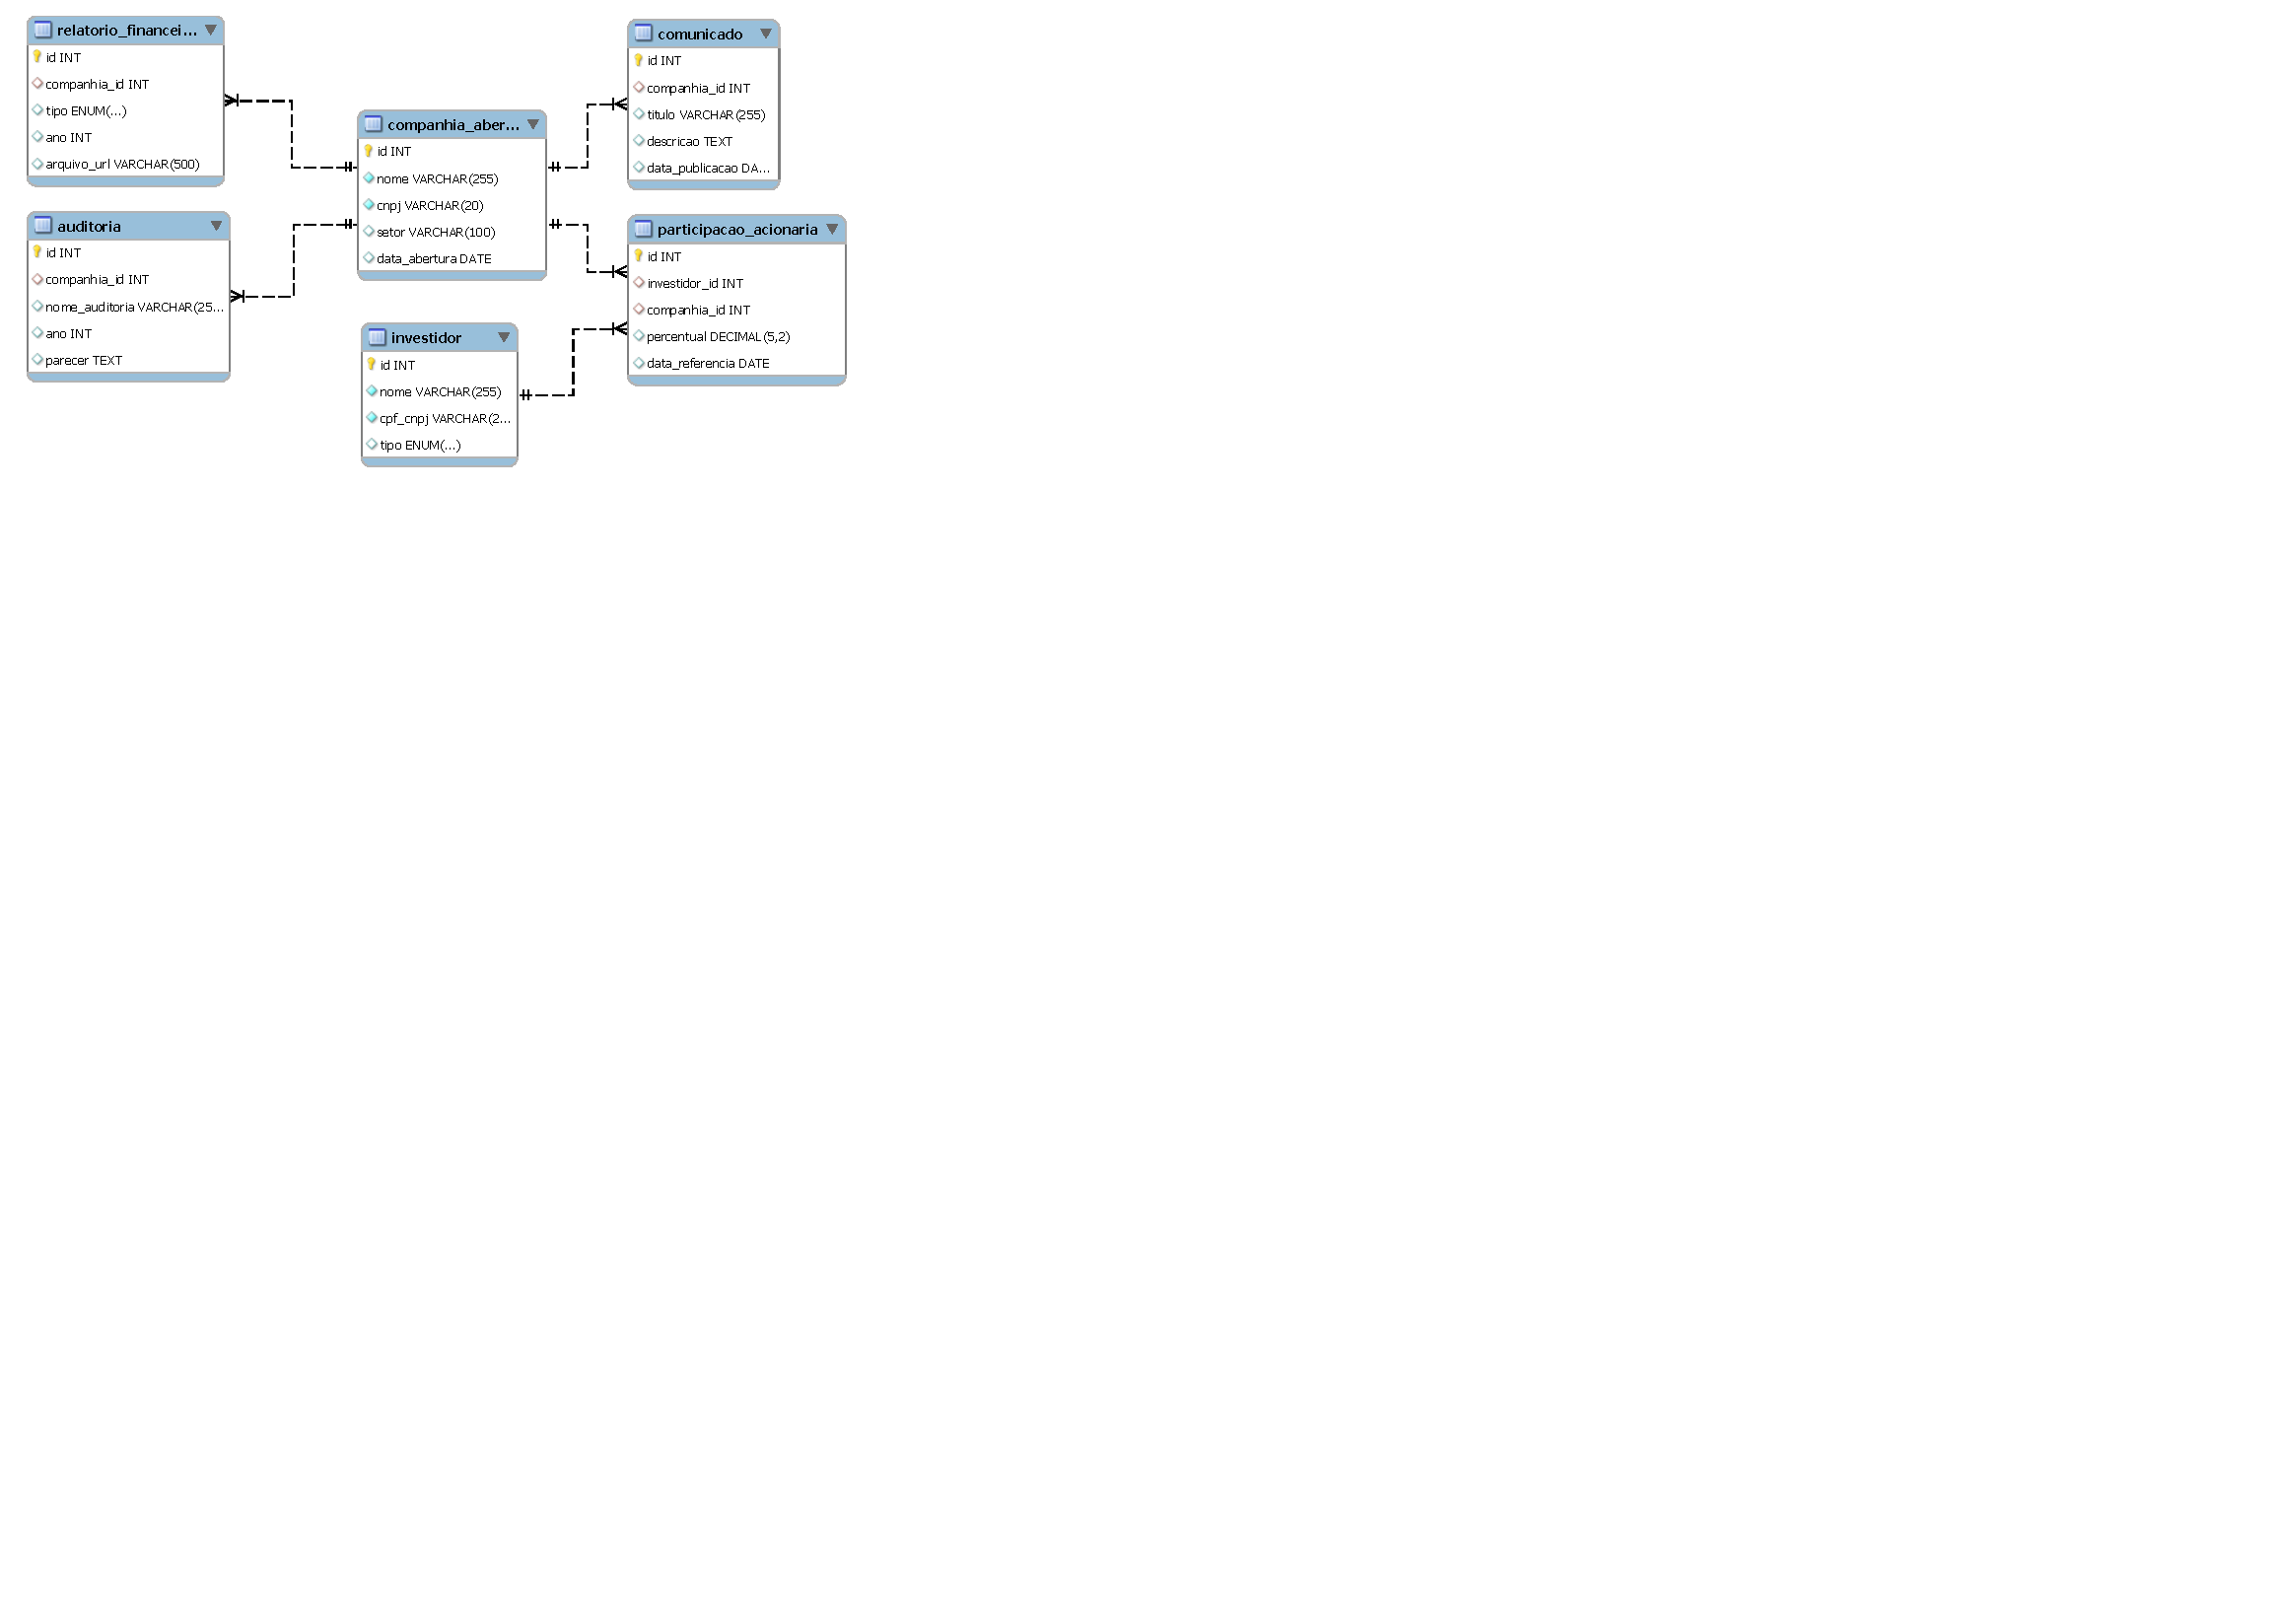
\includegraphics[width=0.9\textwidth]{figuras/esquema_logico.pdf}
	\vspace{1mm}
	\parbox[c]{0.9\textwidth}{\raggedright \legend{Elaborado pelo autor, 2024.}}
\end{figure}

O modelo proposto é composto pelas seguintes tabelas:

\begin{itemize}
	\item \textit{companhia\_aberta}
	\item \textit{comunicado}
	\item \textit{investidor}
	\item \textit{participacao\_acionaria}
	\item \textit{auditoria}
	\item \textit{relatorio\_financeiro}
\end{itemize}

A tabela \textit{companhia\_aberta} centraliza os dados cadastrais das empresas registradas na CVM, contendo atributos como \textit{nome}, \textit{cnpj}, \textit{setor} e \textit{data\_abertura}. O campo \textit{cnpj} possui uma restrição de unicidade (\textit{UNIQUE}) para garantir a integridade dos dados identificadores.

A tabela \textit{comunicado} armazena registros de publicações oficiais vinculadas às companhias, sendo referenciada pela chave estrangeira \textit{companhia\_id}, que estabelece uma relação com a tabela \textit{companhia\_aberta}. Esse vínculo viabiliza a rastreabilidade entre os comunicados e as empresas emissores.

A tabela \textit{investidor} registra os agentes que detêm participações acionárias, identificados pelo atributo \textit{cpf\_cnpj}, e categorizados segundo o tipo de investidor (\textit{Pessoa Física} ou \textit{Pessoa Jurídica}), utilizando a estrutura \textit{ENUM} para controle de domínio.

A tabela \textit{participacao\_acionaria} representa a associação entre investidores e companhias abertas, permitindo o registro da proporção de ações detidas por data de referência. Essa tabela possui chaves estrangeiras para as tabelas \textit{investidor} e \textit{companhia\_aberta}, o que possibilita a análise de composição societária ao longo do tempo.

A tabela \textit{auditoria} documenta os pareceres emitidos por empresas auditoras sobre as demonstrações financeiras das companhias, detalhando o ano do parecer, o nome da auditoria e a descrição do conteúdo emitido.

Por fim, a tabela \textit{relatorio\_financeiro} concentra os metadados dos arquivos financeiros disponibilizados pela CVM, como os Demonstrativos Financeiros Padronizados (DFP), Informações Trimestrais (ITR), o Formulário de Referência e o IAN. Cada registro inclui o tipo do documento, o ano de referência e o link para o arquivo original.

Essa estrutura relacional foi projetada visando à normalização dos dados, conforme as boas práticas de projeto de bancos de dados relacionais \cite{elmasri:2016:fundamentals}. A modelagem lógica aqui apresentada oferece a base necessária para uma integração eficiente e escalável, compatível com análises automatizadas de caráter fundamentalista. Sua implementação favorece a consistência da base de dados, o desempenho nas consultas SQL e a reutilização de componentes em diferentes módulos do sistema.



\subsection{Processo de integração de dados}

A integração de dados é um procedimento essencial que consolida informações oriundas de diversas fontes, garantindo consistência, qualidade e acessibilidade para análises estratégicas e operacionais. Esse processo transforma dados brutos em informações valiosas para a tomada de decisão e é composto por etapas interdependentes: extração, transformação e carga.

Na etapa de extração, os dados são coletados diretamente de múltiplas fontes, como os repositórios da CVM. Essa fase utiliza técnicas que asseguram a captura completa e precisa das informações, minimizando riscos de perda ou corrupção. No presente trabalho, essa etapa foi implementada por meio de \textit{scripts} automatizados em Python, que realizam o download de arquivos compactados disponibilizados pela CVM, como o \texttt{dfp\_cia\_aberta\_2022.zip}. O sistema verifica a existência prévia dos arquivos e sua integridade antes de prosseguir com o processamento, evitando redundâncias e falhas.

Após a extração, os dados brutos passam por um processo de transformação que envolve padronização, limpeza, normalização e aplicação de regras de negócio. Essa etapa é responsável por eliminar inconsistências, corrigir valores ausentes, ajustar formatos e estruturar os dados para análises mais sofisticadas. No contexto deste projeto, foram realizadas conversões de tipos, unificação de formatos de datas e remoção de duplicidades. Informações como o código da conta contábil (\texttt{CD\_CONTA}) foram associadas às suas descrições completas com base nos planos de contas divulgados pela CVM, garantindo maior legibilidade e utilidade analítica.

Na etapa final, os dados transformados são carregados em um banco de dados relacional estruturado, visando facilitar a manipulação, a consulta e a análise posterior. Para este trabalho, optou-se pelo uso do SQLite como solução leve e eficiente, adequada ao escopo local da ferramenta desenvolvida. As tabelas foram criadas respeitando normas de integridade referencial, com chaves primárias e estrangeiras bem definidas. Dados financeiros, cadastrais e operacionais foram organizados em tabelas como \texttt{demonstrativo\_financeiro}, \texttt{informacao\_trimestral} e \texttt{empresas}, possibilitando análises temporais, cálculo de indicadores como LPA e P/L, entre outros.

A integração harmônica dessas etapas resultou em uma base de dados confiável e atualizada, que sustenta a automatização dos processos analíticos e permite a construção de modelos quantitativos e preditivos. Essa abordagem se mostra fundamental para a aplicação da análise fundamentalista no contexto do mercado financeiro, proporcionando uma visão estruturada e estratégica para a tomada de decisão \cite{costa:2024:integraccao, halevy:2006:data}.

\section{Estado da arte} \label{sec:estado-arte}

Nesta seção, são analisados os principais estudos acadêmicos e projetos práticos que fundamentam a abordagem deste trabalho. Inicialmente, apresenta-se uma síntese dos trabalhos existentes, destacando seus objetivos, metodologias empregadas e limitações encontradas. Em seguida, evidencia-se como o presente estudo propõe uma integração inédita de dados e técnicas, superando as deficiências das abordagens anteriores.

\subsection{Trabalhos acadêmicos}

Os estudos acadêmicos voltados à modelagem e à análise de dados financeiros têm se concentrado na automatização da análise fundamentalista e na adaptação de modelos tradicionais ao contexto do mercado brasileiro. Por exemplo, \citet{montoia:2021:automatizaccao} desenvolvem um sistema automatizado para a análise de ações, enfatizando a melhoria na rapidez e na eficiência da tomada de decisões. Esse trabalho detalha a aplicação de algoritmos de processamento de dados que reduzem a intervenção manual, permitindo uma análise em tempo real dos indicadores financeiros.

De forma complementar, \citet{deAraujo:2021:modelo} propôs um modelo flexível que adapta os conceitos da análise fundamentalista para refletir as particularidades dos dados nacionais, considerando variáveis específicas do mercado brasileiro. Esse estudo destaca a importância da customização dos parâmetros e a integração de variáveis macroeconômicas na modelagem financeira.

Além disso, \citet{delalibera:2023:automatizaccao} aprimorou metodologias tradicionais, como o Modelo Rojo, para avaliação de ativos, enfatizando a precisão na quantificação de riscos e oportunidades de investimento. Este trabalho apresenta uma abordagem robusta que combina técnicas estatísticas com algoritmos de \textit{machine learning} para melhorar a acurácia das previsões. Por sua vez, \citet{reis:2020:analise} investigou a aplicação prática desses métodos na análise das ações negociadas, proporcionando \textit{insights} sobre a volatilidade do mercado e a relevância de diferentes indicadores financeiros.

Outros estudos, como o de \citet{vieira:2019:montagem}, analisam estratégias de montagem de carteiras de ações, comparando a performance das carteiras com índices de mercado e ressaltando as dificuldades na diversificação e no balanceamento dos ativos. Da mesma forma, \citet{freitas:2020:analise} explorou a aplicação criteriosa de indicadores no setor bancário, evidenciando os desafios em medir a solidez financeira e a eficiência operacional de instituições financeiras.

\subsection{Projetos e plataformas similares}

No campo dos projetos práticos, diversas iniciativas presentes em repositórios, especialmente no GitHub, vêm se destacando por oferecer ferramentas e bases de dados voltadas para a extração e análise de informações financeiras. Por exemplo, o projeto de \citet{paiva:2025:projetoGitHub} apresenta um sistema integrado que coleta, processa e organiza dados contábeis de empresas. Essa ferramenta tem como objetivo facilitar a aplicação da análise fundamentalista ao disponibilizar dados de forma estruturada e acessível, promovendo maior transparência e facilidade na análise dos balanços.

De maneira similar, \citet{minas:2025:projetoGitHub} propõe uma abordagem inovadora para a análise de balanços empresariais, enfatizando a importância da normalização dos dados e da criação de indicadores personalizados que se ajustem às especificidades de cada setor. Repositórios como os de \citet{fontinele:2025:projetoGitHub} e \citet{louredo:2025:projetoGitHub} se destacam ao desenvolver ferramentas específicas para interpretar demonstrações financeiras a partir de dados públicos, permitindo que o usuário identifique rapidamente pontos críticos e oportunidades de investimento. Contudo, grande parte dessas iniciativas se restringe à coleta e ao processamento dos dados, sem oferecer uma análise histórica contínua que possibilite a compreensão das tendências de longo prazo.

\subsection{Diferencial do trabalho proposto}

O diferencial do presente trabalho reside na integração de um histórico abrangente de dados financeiros com um sistema automatizado de acesso e análise das informações públicas disponibilizadas pela CVM. Embora os experimentos realizados tenham utilizado um recorte temporal de cinco anos, a ferramenta não se limita a esse intervalo. Enquanto a CVM mantiver a estrutura dos dados em seus repositórios, o sistema permanecerá funcional e poderá ser continuamente alimentado com novos dados, garantindo sua atualização e longevidade.

A proposta se distingue, ainda, por tratar-se de uma solução de código aberto, o que permite sua auditoria, personalização e extensão por outros pesquisadores e profissionais interessados. Essa abertura favorece a colaboração contínua, possibilitando o aprimoramento da ferramenta e sua adaptação a novos contextos analíticos ou setores econômicos específicos.

A abordagem adotada neste trabalho viabiliza tanto a avaliação contínua e comparativa dos dados quanto a análise contextualizada das informações. A avaliação contínua é sustentada pelo acúmulo de dados históricos, o que permite identificar tendências e padrões relevantes ao longo do tempo. Já a análise contextualizada emerge da capacidade de combinar dados históricos e atuais, ampliando a compreensão sobre ciclos econômicos, sazonalidades e eventos que impactam o mercado.

As principais inovações e contribuições do sistema desenvolvido podem ser resumidas nos seguintes pontos:

\begin{itemize}
	\item integração de dados históricos financeiros em larga escala;
	\item processamento automatizado, com foco em escalabilidade e reusabilidade;
	\item contextualização dos indicadores contábeis e financeiros;
	\item manutenção da funcionalidade do sistema diante de novas atualizações da CVM, desde que preservada a estrutura de dados;
	\item disponibilização em formato de código aberto, fomentando a transparência e a colaboração.
\end{itemize}

Ao superar as limitações de iniciativas anteriores, que se restringem majoritariamente à coleta e estruturação pontual dos dados, a solução apresentada promove uma abordagem sistemática e extensível, capaz de subsidiar análises fundamentalistas robustas e atualizadas. Essa característica torna o sistema especialmente útil para aplicações acadêmicas, institucionais e profissionais voltadas à tomada de decisão baseada em fundamentos econômicos e financeiros.

\chapter{METODOLOGIA}

 Esta seção apresenta a metodologia de execução do presente trabalho.
A Seção \ref{subsec:classificacao} define o escopo e os objetivos deste trabalho, delineando as principais áreas de investigação.
Em seguida, a Seção \ref{subsec:metodologia} descreve as abordagens e técnicas utilizadas para planejar e conduzir o desenvolvimento da ferramenta proposta.
Por fim, a Seção \ref{subsec:solucao} detalha os passos do trabalho, incluindo a investigação da estrutura dos dados, a modelagem lógica e o desenvolvimento da ferramenta de integração de dados.

\section{Classificação da Pesquisa} \label{subsec:classificacao}

Para fundamentar a classificação metodológica da pesquisa, foram consultadas as obras de \citet{cervo:1983:metodologia}, que apresentam diferentes abordagens científicas, e de \citet{gerhardt:2009:metodos}, que tratam de métodos amplamente utilizados na pesquisa acadêmica.

Quanto à natureza, esta pesquisa é aplicada, pois busca resolver um problema prático relacionado à integração automatizada de dados financeiros públicos disponibilizados pela CVM, promovendo avanços na análise fundamentalista e no apoio à tomada de decisão.

Em relação aos objetivos, a investigação é exploratória e descritiva. A parte exploratória está ligada à compreensão da estrutura dos dados da CVM, enquanto o aspecto descritivo se manifesta na proposição e implementação de uma ferramenta que permita o uso prático dessas informações de forma organizada.

Os procedimentos técnicos combinam pesquisa bibliográfica e documental para levantamento e compreensão teórica dos dados públicos, juntamente com o desenvolvimento de uma solução tecnológica que automatiza sua coleta, integração e disponibilização.

A abordagem metodológica adotada é mista. Aspectos qualitativos estão presentes na análise estrutural e na modelagem dos dados, enquanto os elementos quantitativos se refletem no processamento automatizado e na organização das informações em larga escala.

No contexto da área de Computação, a pesquisa representa o desenvolvimento de uma solução tecnológica voltada à resolução de um problema específico, com potencial de aplicação prática no meio acadêmico e no ambiente de análise financeira \cite{wazlawick:2009:metodo}.


\section{Gerenciamento do Projeto} \label{subsec:metodologia}

O gerenciamento deste projeto foi conduzido com base em práticas ágeis de desenvolvimento de software, adotando a metodologia \textit{Scrum} como estrutura principal \cite{schwaber:2004:agile}. Como apoio visual, utilizou-se também o quadro de sinalização \textit{Kanban}, contribuindo para a organização e o acompanhamento do fluxo de trabalho \cite{anderson:2010:kanban}.

Ambas as abordagens foram aplicadas de forma adaptada às necessidades do projeto, considerando sua natureza acadêmica e o escopo restrito da equipe envolvida. O \textit{Scrum} foi utilizado de maneira personalizada, com ciclos iterativos de duas semanas, denominados \textit{sprints}, nos quais as tarefas foram definidas, priorizadas e acompanhadas ao longo do desenvolvimento \cite{sutherland:2014:scrum}.

O Kanban complementou esse processo, funcionando como ferramenta visual para monitoramento das atividades, identificação de gargalos e ajustes de fluxo, contribuindo para uma gestão mais eficiente \cite{hammarberg:2014:kanban}. Essa combinação flexível e adaptada de métodos ágeis mostrou-se eficaz para garantir a organização, a visibilidade do progresso e a entrega incremental da solução proposta.



\section{Solução proposta}  \label{subsec:solucao}

O ponto de partida do projeto consistiu em uma investigação detalhada da estrutura dos dados disponibilizados pela CVM. Essa etapa contemplou a análise dos formatos de arquivos, dos tipos de dados disponíveis e dos métodos de acesso às informações públicas fornecidas por essa instituição.

Embora os dados da B3 não tenham sido utilizados diretamente na construção da ferramenta, sua presença no contexto do mercado de capitais justificou a compreensão de sua estrutura e funcionamento. Dessa forma, foram consultados documentos como o relatório anual da CVM \cite{cvm:2023:relatorioanual} e referências sobre a estrutura de dados da B3 \cite{b3:2023:estruturadados}, a fim de mapear desafios e possibilidades associados à integração de dados financeiros.

A Figura \ref{fig:fluxograma} ilustra o fluxo geral do projeto. A fase inicial compreendeu a coleta e documentação dos dados da CVM, seguida pela modelagem lógica que estruturou um banco de dados unificado, preparado para integração e análise posterior.

\begin{figure}[!htb] \centering
	\caption{Fluxograma do projeto} \label{fig:fluxograma}
	\begin{varwidth}{\linewidth}
		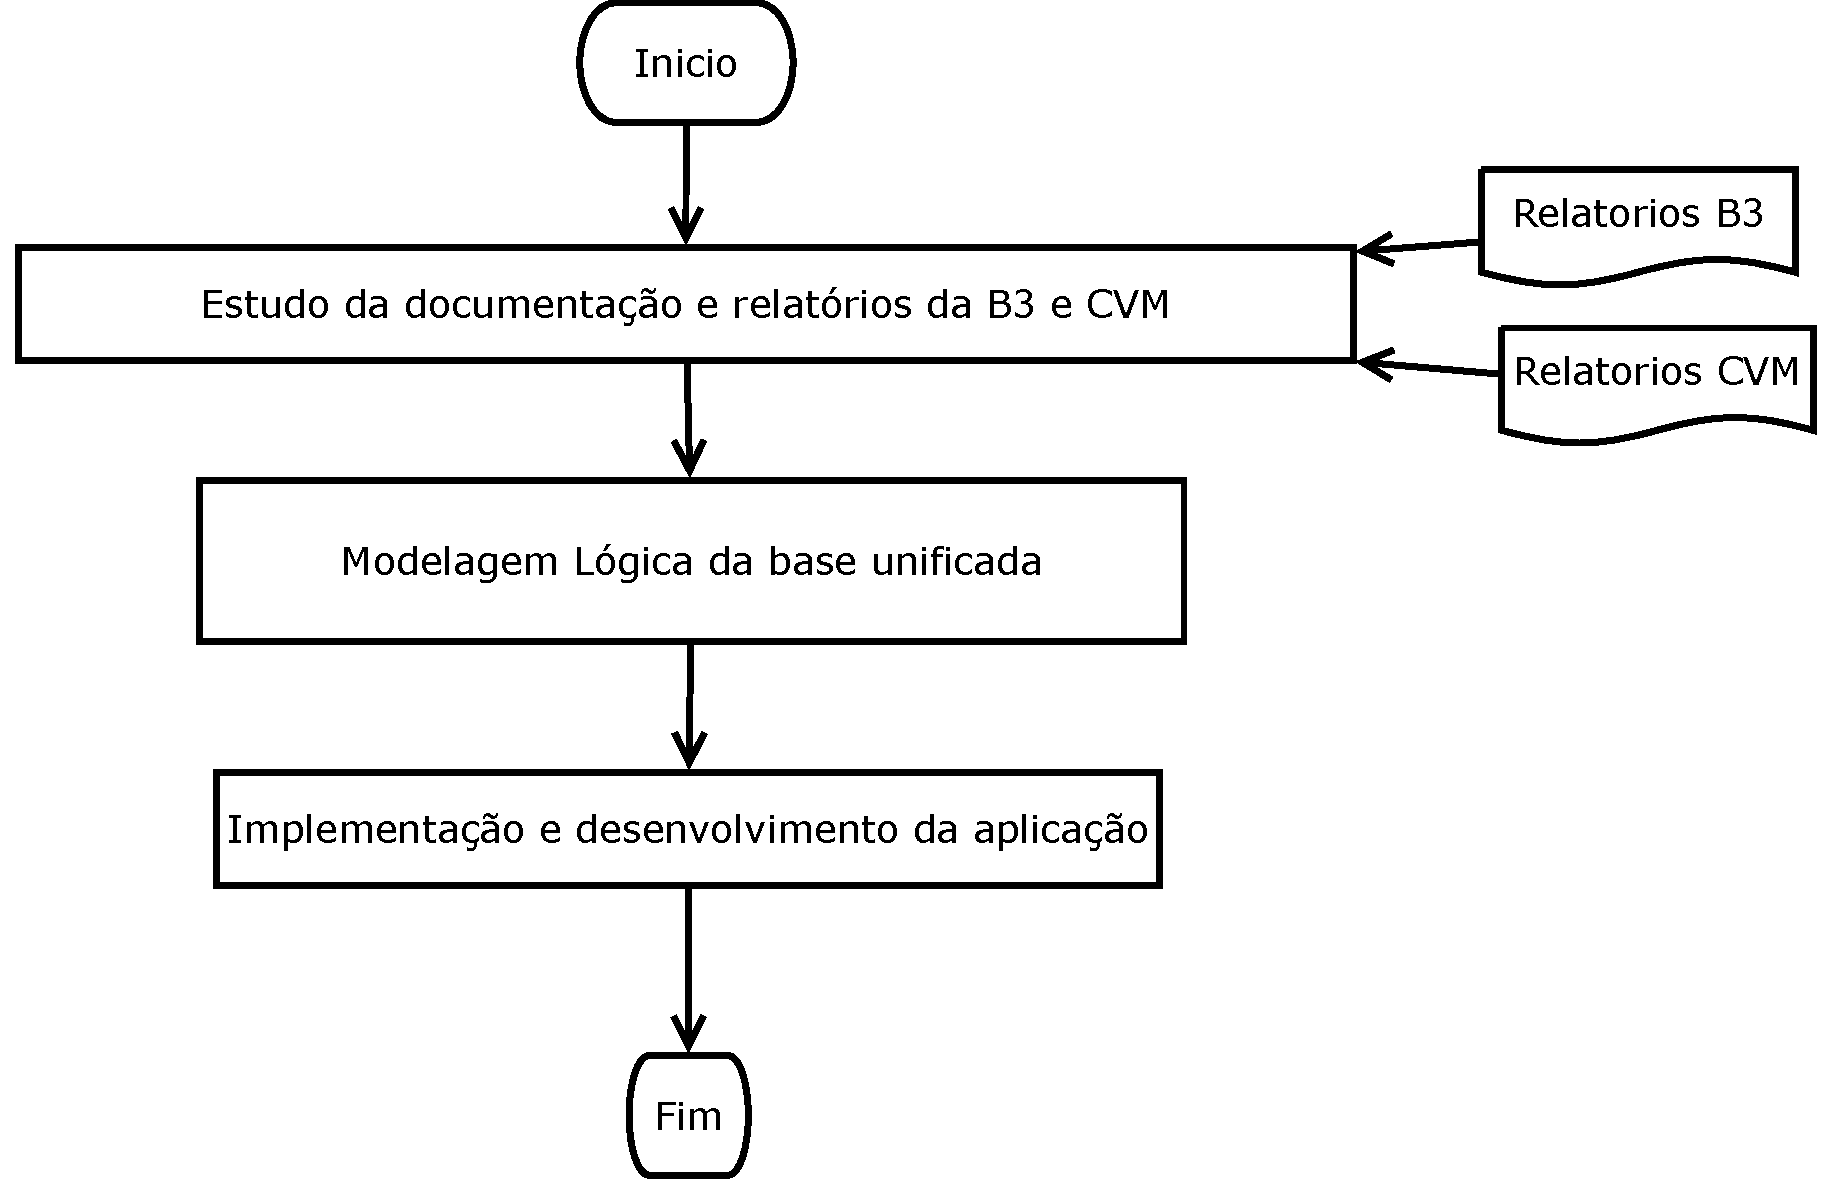
\includegraphics[width=0.6\textwidth]{figuras/fluxograma - v3.pdf}
		\legend{Elaborado pelo autor, 2024.}
	\end{varwidth}
\end{figure}

Com base na análise inicial, foi realizada a modelagem lógica da base de dados, com foco na criação de um esquema unificado que contemplasse as diferentes estruturas contábeis e financeiras presentes nos arquivos da CVM. Para essa etapa, foram consideradas boas práticas descritas na literatura sobre modelagem de dados financeiros \cite{domingues:2020:modelagem} e integração de grandes volumes de dados \cite{perlin:2021:analise}.

A etapa seguinte consistiu no desenvolvimento da aplicação de software responsável por automatizar o processo de coleta, tratamento e inserção dos dados na base unificada. Essa ferramenta foi desenvolvida com tecnologias modernas de extração e processamento de dados, garantindo flexibilidade e desempenho.

A aplicação foi capaz de realizar o download dos arquivos disponibilizados pela CVM, aplicar os tratamentos necessários para padronização e limpeza dos dados, e armazená-los de forma estruturada. Esse processo assegurou a integridade das informações e facilitou seu uso em análises fundamentalistas, estudos acadêmicos e outras aplicações. A proposta esteve alinhada com práticas consolidadas no desenvolvimento de soluções para automação e análise de dados \cite{prikladnicki:2014:desenvolvimentosoftware} \cite{nhimi:2016:desenvolvimentosoftware}.


\section{Materiais e Tecnologias} \label{subsec:material}

Esta seção apresenta os materiais e tecnologias que serão empregados durante o desenvolvimento do trabalho.  
O projeto será desenvolvido em um computador desktop cujas especificações são apresentadas no Quadro \ref{tab:specs-tcc}.  


\begin{board}[!htb]  \centering
	\caption{Especificações do computador utilizado no TCC}
	\label{tab:specs-tcc}
	\begin{varwidth}{\linewidth}
		\begin{tabular}{|p{4cm}|p{11cm}|} \hline
			\textbf{Componente} & \textbf{Especificação} \\ \hline
			Processador & AMD Ryzen 5 5600G, 6-Core, 12-Threads, 3.6GHz (4.6GHz Turbo), Cache 19MB, AM4 \\ \hline  
			Memória RAM & 2x Kingston Fury Beast, 16GB, 3200MHz, DDR4, CL16 \\ \hline  
			Armazenamento & SSD TGT Seal ST, 240GB, Sata III, Leitura 500 MB/s, Gravação 450 MB/s \\  
			& HD WD Blue, 1TB, 3.5, 5400 RPM, Sata III, Cache 64MB \\ \hline  
			Sistema Operacional & Windows 11 Pro \\ \hline
		\end{tabular}
		\legend{Elaborado pelo autor, 2024.}
	\end{varwidth}
\end{board}

Durante a modelagem do banco de dados, utilizou-se o MySQL Workbench\footnote{\url{https://www.mysql.com/products/workbench/}}, versão 8.0. Essa ferramenta permitiu a criação visual do esquema lógico, facilitando o planejamento e a organização das entidades e relacionamentos.

Contudo, para o desenvolvimento da aplicação, optou-se pelo uso do SQLite\footnote{\url{https://www.sqlite.org/}}, versão 3.49.1, como solução de banco de dados local. O SQLite foi adotado como banco de dados padrão do sistema, por oferecer maior praticidade na integração com o código desenvolvido. Sua leveza, portabilidade e independência de um servidor o tornam especialmente adequado para o uso do código por estudantes e profissionais da área financeira.

A linguagem de programação utilizada foi o Python, na versão 3.12.9\footnote{\url{https://www.python.org/downloads/release/python-3129/}}, pela sua versatilidade, ampla comunidade e bibliotecas especializadas.

As bibliotecas utilizadas no projeto foram:

\begin{itemize}
	\item Pandas, versão 2.2.1\footnote{\url{https://pandas.pydata.org/}}
	\item Numpy, versão 1.26.4\footnote{\url{https://numpy.org/}}
	\item Beautifulsoup4, versão 4.12.2\footnote{\url{https://www.crummy.com/software/BeautifulSoup/}}
	\item Lxml, versão 5.1.0\footnote{\url{https://lxml.de/}}
	\item Requests, versão 2.31.0\footnote{\url{https://requests.readthedocs.io/en/latest/}}
	\item SQLAlchemy, versão 2.0.27\footnote{\url{https://www.sqlalchemy.org/}}
	\item Mysql-Connector-Python, versão 8.3.0\footnote{\url{https://dev.mysql.com/downloads/connector/python/}}
\end{itemize}

A biblioteca \textit{pandas} foi empregada para manipulação e análise de dados tabulares. Sua estrutura baseada em \textit{DataFrames} proporcionou uma forma eficiente de organizar, filtrar e agrupar informações financeiras.

A biblioteca \textit{numpy} foi utilizada em conjunto com o pandas para operações numéricas vetoriais e matriciais, fundamentais na realização de cálculos e no tratamento de grandes volumes de dados.

Para extração de informações de páginas web, foi utilizada a biblioteca \textit{beautifulsoup4}, que permitiu navegar pela estrutura HTML de documentos e extrair dados de forma precisa. A ela foi integrada a biblioteca \textit{lxml}, que serviu como parser rápido e eficiente de HTML e XML.

A coleta dos dados disponibilizados pela CVM foi realizada por meio da biblioteca \textit{requests}, que viabilizou a comunicação com serviços HTTP e o download automatizado das informações necessárias.

A interface com o banco de dados foi desenvolvida com o auxílio do \textit{SQLAlchemy}, que forneceu abstração e controle sobre as operações de inserção, consulta e atualização dos dados no SQLite, utilizando o paradigma de mapeamento objeto-relacional.

%Texto antigo
%Durante os testes iniciais com a estrutura modelada no MySQL, foi utilizada a biblioteca \textit{mysql-connector-python}, o conector oficial do MySQL para Python. Essa ferramenta garantiu a compatibilidade entre a modelagem relacional inicial e os scripts desenvolvidos, possibilitando a validação funcional da estrutura antes da migração definitiva para o SQLite.
%
%A escolha pelo banco de dados SQLite justifica-se por sua leveza, portabilidade e facilidade de integração com sistemas locais, características adequadas a estudos exploratórios e reprodutíveis.

%Texto novo
Durante a fase inicial de testes com a estrutura relacional modelada em MySQL, utilizou-se a biblioteca \textit{mysql-connector-python}, conector oficial disponibilizado para integração entre aplicações Python e bancos de dados MySQL. Essa ferramenta assegurou plena compatibilidade entre o modelo relacional e os \textit{scripts} desenvolvidos, permitindo validar o funcionamento da estrutura proposta em um ambiente robusto e amplamente utilizado no contexto de bancos relacionais.

Após essa etapa de validação, optou-se pela migração definitiva para o banco de dados SQLite. A escolha por essa tecnologia deve-se à sua leveza, portabilidade e facilidade de integração com sistemas locais, características particularmente vantajosas para estudos exploratórios, reproduzíveis e com foco acadêmico ou experimental, como é o caso deste trabalho.

%TODO - a mexer
\chapter{DESENVOLVIMENTO}

Este capítulo apresenta o processo de desenvolvimento da ferramenta proposta para a coleta, estruturação e integração de dados financeiros públicos disponibilizados pela CVM, com foco em análises fundamentalistas de companhias abertas brasileiras.

As atividades foram organizadas em três frentes principais, que estruturam as seções deste capítulo. A Seção~\ref{sec:analise_cvm} descreve a análise preliminar dos dados disponibilizados pela CVM, com destaque para a identificação de padrões, inconsistências e limitações nos metadados. A Seção~\ref{sec:modelagem} detalha a modelagem e estruturação da base de dados, com ênfase na padronização relacional e na aplicação de boas práticas de modelagem para contextos financeiros, conforme discutido na literatura \cite{elmasri:2016:fundamentals}. Por fim, a Seção~\ref{sec:software} apresenta o sistema desenvolvido em Python, incluindo os módulos responsáveis pela coleta, transformação e armazenamento dos dados, bem como os mecanismos de registro de eventos (\textit{logs}).


\section{Análise inicial dos dados da CVM} \label{sec:analise_cvm}

A primeira etapa consistiu na compreensão do formato, da frequência de atualização e de outros aspectos relevantes relacionados aos dados disponibilizados pela CVM com foco do trabalho são as Companhias (CIA) Abertas. A partir disso, foram identificados os conjuntos de dados referentes às Companhias Abertas, organizados nas seguintes pastas:

\begin{itemize}
	\item informação cadastral;
	\item formulário cadastral;
	\item informações periódicas e eventuais;
	\item formulário de referência;
	\item valores mobiliários negociados e detidos;
	\item formulário de informações trimestrais;
	\item formulário de demonstrações financeiras padronizadas;
	\item informe do código de governança.
\end{itemize}

As informações cadastrais compõem uma categoria distinta, classificada como cadastro, enquanto os demais arquivos são agrupados sob a categoria de documentos. Ao acessar o site de dados da CVM\footnote{\url{https://dados.cvm.gov.br/dados/}}, especificamente a seção referente às Companhias Abertas, é possível visualizar essas duas categorias de dados.

Adicionalmente, é importante contextualizar o sistema responsável pelo envio eletrônico dos documentos à CVM. O sistema \textit{Empresas.NET} (ENET) é a plataforma oficial utilizada pelas companhias abertas para a transmissão de informações regulatórias exigidas pela autarquia. Essa ferramenta garante a padronização, segurança e rastreabilidade do envio, sendo o meio exclusivo de entrega de documentos previstas nas normas vigentes.

Os dados disponibilizados no portal da CVM são disponibilizados em formatos estruturados em \textit{Comma-Separated Values} (CSV, em português valores separados por vírgulas), em texto simples no formato \texttt{TXT} e arquivos comprimidos no formato \texttt{ZIP}. Esses formatos visam garantir maior acessibilidade e automação no tratamento das informações. A maioria dos conjuntos de dados está organizada em arquivos anuais, separados por tipo de formulário e data de referência, o que permite consultas retroativas e reprodutibilidade dos resultados.

Essas pastas listadas anteriormente podem conter dados referentes à categoria principal ou subdivisões internas em (subcategorias), conforme a complexidade do conteúdo. Os metadados associados a cada categoria são apresentados de duas formas. Quando não há subcategorias, os metadados são oferecidos em arquivos de texto; caso contrário, são fornecidos em arquivos compactados que, ao serem descompactados, revelam arquivos textuais para cada subcategoria.

%Os dados propriamente ditos também são disponibilizados em arquivos compactados por ano. Após a extração, o conteúdo pode variar: em categorias sem subdivisões, o arquivo anual tende a conter um único documento estruturado; já em categorias com subcategorias, o arquivo anual inclui múltiplos arquivos estruturado, organizados conforme os diferentes tipos de informação tratados.
%
%Dessa forma, observa-se um padrão de organização hierárquica: pastas por categoria principal, contendo arquivos de metadados e dados, com granularidade ajustada conforme a existência de subcategorias. Essa estrutura visa facilitar o acesso modular à informação alem de um controle sobre a atualização dos dados e permitir análises específicas com base no ano.
%
%As legislações que fundamentam a disponibilização e a estrutura dos dados incluem, principalmente, a Resolução CVM nº 80/2022 \cite{cvm:2022:resolucao80}, que consolida as regras relativas ao registro e envio de informações pelas companhias abertas, e a Resolução CVM nº 44/2021 \cite{cvm:2021:resolucao44}, que dispõe sobre a divulgação de informações relativas a atos ou fatos relevantes, a negociação de valores mobiliários na pendência de tais informações ainda não divulgadas, bem como sobre a divulgação de operações realizadas com valores mobiliários por pessoas com acesso a informações privilegiadas. Tais normas conferem respaldo jurídico à padronização e à publicidade dos dados disponibilizados, sendo essenciais para o desenvolvimento de sistemas automatizados de análise fundamentada, como o proposto neste trabalho.

Os dados propriamente ditos também são disponibilizados em arquivos compactados por ano. Após a extração, o conteúdo pode variar: em categorias sem subdivisões, o arquivo anual tende a conter um único documento estruturado; já em categorias com subcategorias, o arquivo anual inclui múltiplos arquivos estruturados, organizados conforme os diferentes tipos de informação tratados.

Dessa forma, observa-se um padrão de organização hierárquica: pastas por categoria principal, contendo arquivos de metadados e dados, com granularidade ajustada conforme a existência de subcategorias. Essa estrutura visa facilitar o acesso modular à informação, além de permitir maior controle sobre a atualização dos dados e a realização de análises específicas com base no ano.

A disponibilização e estruturação dos dados têm como base legal a Resolução CVM nº 80/2022~\cite{cvm:2022:resolucao80}, que consolida as regras relativas ao registro e envio de informações pelas companhias abertas, e a Resolução CVM nº 44/2021~\cite{cvm:2021:resolucao44}, que dispõe sobre a divulgação de informações relativas a atos ou fatos relevantes, a negociação de valores mobiliários na pendência dessas informações ainda não divulgadas, bem como sobre a divulgação de operações realizadas por pessoas com acesso a informações privilegiadas.

Tais normas conferem respaldo jurídico à padronização e à publicidade dos dados disponibilizados. Além disso, tornam-se essenciais para a implementação de sistemas automatizados de análise fundamentada, como o proposto neste trabalho, uma vez que garantem consistência normativa e previsibilidade no tratamento da informação.


%Resolução cvm:2022:resolucao
%Resolução cvm:2021:resolucao44

\subsection{Informação cadastral} 

%O conjunto Informação Cadastral reúne os dados cadastrais das companhias abertas disponibilizados pela CVM. Entre as informações disponibilizadas, destacam-se o número do Cadastro Nacional da Pessoa Jurídica (CNPJ), a data de registro da companhia e a situação atual desse registro. Esses dados são fundamentais para análises regulatórias, econômicas e financeiras, além de servirem como base para estudos acadêmicos e pesquisas de mercado. O dicionário de dados, disponibilizado em formato textual, contém a descrição detalhada das colunas e dos tipos de dados presentes no arquivo principal. Já os dados propriamente ditos, que contêm os registros cadastrais das companhias abertas, são apresentados em um arquivo estruturado.

O conjunto de informação cadastral reúne os dados cadastrais das companhias abertas disponibilizados pela CVM. Entre as informações fornecidas, destacam-se o número do Cadastro Nacional da Pessoa Jurídica (CNPJ), a data de registro da companhia e a situação atual desse registro.

Esses dados são fundamentais para análises regulatórias, econômicas e financeiras, além de servirem como base para estudos acadêmicos e pesquisas de mercado. A padronização e a disponibilidade pública dessas informações ampliam a transparência e favorecem o desenvolvimento de soluções automatizadas voltadas à análise institucional das companhias.

O dicionário de dados, disponibilizado em formato textual, contém a descrição detalhada das colunas e dos tipos de dados presentes no arquivo principal. Já os dados propriamente ditos, que contêm os registros cadastrais das companhias abertas, são apresentados em um arquivo estruturado.

Embora o conjunto de informações cadastrais não tenha sido utilizado diretamente nas etapas de extração, modelagem ou análise do presente trabalho, sua estrutura é apresentada a seguir com o intuito de ilustrar o escopo e a organização dos dados disponibilizados pela CVM. A Tabela~\ref{tab:exemplo_informacao_cadastral} mostra uma amostra simplificada desses registros, destacando alguns dos campos mais representativos, como a razão social, o CNPJ, a situação cadastral, o setor de atuação e o endereço eletrônico da companhia.

\begin{table}[!htb]
	\centering
	\caption{Exemplo de registros da base Informação Cadastral}
	\label{tab:exemplo_informacao_cadastral}
	\scriptsize
	\begin{tabularx}{\textwidth}{|X|X|X|X|X|X|X|}
		\hline
		\textbf{CNPJ\_CIA} & \textbf{DENOM\_SOCIAL} & \textbf{DT\_REG} & \textbf{SIT} & \textbf{CD\_CVM} & \textbf{SETOR\_ATIV} & \textbf{EMAIL} \\
		\hline
		08.773.135/0001-00 & 2W ECOBANK S.A. - EM RECUPERAÇÃO JUDICIAL & 29/10/2020 & ATIVO & 25224 & Energia Elétrica & ri@2wecobank.com.br \\
		\hline
		11.396.633/0001-87 & 3A COMPANHIA SECURITIZADORA & 08/03/2010 & CANCELADA & 21954 & Securitização de Recebíveis & dri@3asec.com.br \\
		\hline
		01.547.749/0001-16 & 521 PARTICIPAÇÕES S.A. - EM LIQUIDAÇÃO EXTRAJUDICIAL & 11/07/1997 & ATIVO & 16330 & Emp. Adm. Part. - Energia Elétrica & eximia@eximiacapital.com \\
		\hline
		01.851.771/0001-55 & 524 PARTICIPAÇÕES SA & 30/05/1997 & ATIVO & 16284 & Emp. Adm. Part. - Sem Setor Principal & gar@opportunity.com.br \\
		\hline
	\end{tabularx}
	\legend{Fonte: Dados abertos da CVM (adaptado pelo autor, 2025).}
\end{table}

Além da amostra apresentada, com o objetivo de oferecer uma visão mais abrangente da estrutura do conjunto, apresenta-se no Apêndice~\ref{ap:estrutura-informacao-cadastral} uma tabela-resumo contendo a descrição completa dos campos disponíveis no arquivo principal. Essa estrutura complementar contribui para contextualizar o nível de detalhamento e a organização dos dados, mesmo não sendo incorporados às etapas analíticas deste trabalho.


\subsection{Formulário cadastral}

O formulário cadastral (FCA) é um documento eletrônico cuja entrega periódica ou eventual é regulamentada pelo a CVM e suas resoluções. Este formulário deve ser enviado à CVM por meio do sistema ENET, sendo uma obrigação regulatória destinada às companhias abertas. Sua principal função é atualizar e manter organizadas as informações institucionais e operacionais dessas entidades. O conjunto de dados públicos relacionados ao FCA, disponibilizado pela CVM, apresenta-se organizado em duas categorias principais de informações: os endereços de \textit{download} dos documentos completos submetidos pelas companhias abertas e os conteúdos estruturados das seções que compõem o formulário.

Seguindo o padrão já apresentando de subcategorias o FCA possui a categoria refere-se ao arquivo \texttt{fca\_cia\_aberta}, que contém os links para o \textit{download} dos documentos completos entregues pelas companhias nos últimos cinco anos. A visualização desses documentos requer a utilização do ENET. A as demais categorias compreende os conteúdos integrais do formulário, apresentados abaixo em arquivos estruturados por ano, estando dentro de um arquivo compactado por ano, conforme ja relatado anteriormente. 

A Figura~\ref{fig:estrutura_fca} ilustra de forma resumida a estrutura interna dessa categoria, destacando os arquivos que foram de fato utilizados na análise. Os demais arquivos, não essenciais para este trabalho, foram omitidos por brevidade.

\begin{figure}[!htb]
	\centering
	\caption{Estrutura resumida da categoria FCA}
	\label{fig:estrutura_fca}
	\begin{varwidth}{\linewidth}
		\dirtree{%
			.1 {fca\_cia\_aberta}.
			.2 {fca\_cia\_aberta.csv} \DTcomment{links ENET}.
			.2 {fca\_cia\_aberta\_geral.csv} \DTcomment{dados estruturados}.
			.2 {fca\_cia\_aberta\_auditor.csv}.
			.2 {fca\_cia\_aberta\_valor\_mobiliario.csv}.
			.2 {[... outros arquivos estruturados omitidos]}.
		}
		\legend{Elaborado pelo autor, 2025.}
	\end{varwidth}
\end{figure}

Cada um desses arquivos aborda uma seção específica do formulário, possibilitando a segmentação e a análise detalhada das informações declaradas pelas companhias abertas Uma visão geral dos arquivos estruturados do FCA, com a respectiva correspondência normativa e observações de uso, está apresentada no Apêndice~\ref{ap:estrutura-fca}. Os arquivos são atualizados semanalmente, refletindo tanto novas entregas quanto reapresentações realizadas pelas companhias reguladas. Além disso, mantém-se um histórico contínuo desde o ano de 2010, incluindo inclusive arquivos que não estão sujeitos à política de atualização vigente. O dicionário de dados correspondente é disponibilizado em formato compactado e oferece descrições de todas as colunas e variáveis presentes nos arquivos.

No desenvolvimento da ferramenta proposta neste trabalho, foi utilizado exclusivamente o arquivo \texttt{fca\_cia\_aberta\_geral}, por concentrar de forma consolidada as principais informações institucionais das companhias abertas, o que dispensa a necessidade de integrar os demais arquivos individualizados.

Para exemplificar a estrutura e o conteúdo desses dados, a Tabela~\ref{tab:amostra_fca} apresenta uma amostra representativa de registros extraídos da versão mais recente do conjunto. Esses dados concentram as principais informações institucionais das companhias abertas, como CNPJ, razão social, data de constituição, categoria e situação do registro na CVM, setor de atuação e endereço eletrônico. Tal amostra evidencia o caráter consolidado do arquivo, o que reforça sua escolha como fonte principal para o desenvolvimento da ferramenta proposta neste trabalho.


\begin{table}[!htb]
	\centering
	\caption{Amostra de registros do arquivo \texttt{fca\_cia\_aberta\_geral}}
	\label{tab:amostra_fca}
	\scriptsize
	\begin{tabularx}{\textwidth}{|l|c|c|X|X|c|c|c|X|X|}
		\hline
		\textbf{CNPJ} & \textbf{Ref.} & \textbf{Versão} & \textbf{Empresa} & \textbf{Nome Anterior} & \textbf{Constituição} & \textbf{Categoria} & \textbf{Situação} & \textbf{Setor} & \textbf{Website} \\
		\hline
		00.000.000/0001-91 & 01/01/2025 & 1 & BCO BRASIL S.A. & --- & 12/10/1808 & A & Ativo & Banco Múltiplo & www.bb.com.br \\
		\hline
		00.000.208/0001-00 & 01/01/2025 & 2 & BRB BANCO DE BRASÍLIA S.A. & BANCO REGIONAL DE BRASÍLIA S.A. - BRB & 10/12/1964 & A & Ativo & Banco Múltiplo & www.brb.com.br \\
		\hline
		00.001.180/0001-26 & 01/01/2025 & 2 & CENTRAIS ELÉT. BRAS. S.A. - ELETROBRAS & --- & 11/06/1962 & A & Ativo & Holding de Energia & www.eletrobras.com \\
		\hline
	\end{tabularx}
	\legend{Fonte: Dados abertos da CVM (adaptado pelo autor, 2025).}
\end{table}


Para fins de análise temporal e organização, os formulários referentes aos anos de 2020 a 2025 encontram-se agrupados em arquivos anuais distintos. Este conjunto de dados integra a base denominada \textit{Documentos Periódicos e Eventuais de Regulados}. Sua manutenção ocorre de forma semanal, assegurando a atualização constante das informações disponibilizadas.

\subsection{Informações periódicas e eventuais}

O conjunto de dados referente às informações periódicas e eventuais (IPE) reúne documentos não estruturados enviados por companhias abertas à CVM. Esses documentos, de caráter regulatório, contemplam tanto as obrigações periódicas quanto as comunicações eventuais exigidas ao longo das atividades societárias e da interlocução com o mercado. Trata-se de um acervo, que reflete a diversidade de exigências legais e normativas aplicáveis às companhias reguladas. O conteúdo do conjunto está organizado em seis grandes categorias documentais:

\begin{itemize}
	\item governança e estrutura societária;
	\item relação com investidores e mercado;
	\item informações econômico-financeiras e contábeis;
	\item transações e operações societárias;
	\item companhias em situação especial;
	\item informações regulatórias específicas.
\end{itemize}

Uma visão geral dos tipos documentais abrangidos pelo conjunto IPE pode ser consultada no Apêndice~\ref{ap:ipe-visao-geral}.

%A categoria de governança e estrutura societária compreende documentos que regulam a organização interna e as diretrizes de conduta das companhias, como Acordos de Acionistas, Estatutos Sociais, Regimentos Internos, Códigos de Conduta, além de Políticas de Governança e Sustentabilidade. Esses registros são fundamentais para garantir a conformidade, a transparência e a integridade das práticas de gestão corporativa. 
%
%Já os documentos de relação com investidores e mercado incluem comunicados oficiais direcionados ao público investidor e à sociedade, como Comunicados ao Mercado, Avisos a Acionistas e Debenturistas, Fatos Relevantes, Informações prestadas a bolsas estrangeiras e o Calendário de Eventos Corporativos. Tais documentos asseguram a divulgação tempestiva e adequada de informações relevantes, conforme exigido pelas normas da CVM.
%
%No que se refere às informações econômico-financeiras e contábeis, o conjunto abrange dados sobre a situação patrimonial e os resultados das companhias, além de instrumentos financeiros e políticas de distribuição de lucros. Incluem-se nessa categoria Demonstrativos Financeiros, Documentos de Ofertas Públicas, Escrituras de Debêntures, Políticas de Dividendos e de Destinação de Resultados. A categoria de transações e operações societárias, por sua vez, contém registros de eventos relevantes que impactam a estrutura e o capital das empresas, como Comunicações sobre Transações com Partes Relacionadas, Ofertas Públicas de Aquisição (OPA) e Planos de Remuneração Baseados em Ações. 
%
%Já a documentação relativa a companhias em situação especial reúne informações sobre empresas que enfrentam processos de falência, liquidação ou recuperação judicial/extrajudicial, sendo essenciais para análise de risco e monitoramento da situação jurídico-financeira dessas entidades. Por fim, a categoria de informações regulatórias específicas abrange documentos exigidos por normativos da CVM, como as comunicações sobre negociação de valores mobiliários por pessoas ligadas, políticas de atuação de auditores independentes e outras políticas internas obrigatórias.
%
%Todos os documentos do conjunto IPE são disponibilizados em arquivos compactados organizados por ano, mesmo quando cada compactado contém apenas um único arquivo estruturado em seu interior. Os arquivos correspondentes ao ano corrente e ao ano imediatamente anterior são atualizados semanalmente, incorporando tanto novas submissões quanto eventuais reapresentações. O acervo possui cobertura histórica desde 2003, incluindo arquivos legados que, embora não estejam sujeitos à política atual de atualização contínua, permanecem acessíveis para consulta.
%
%Cada conjunto anual acompanha um arquivo auxiliar contendo o dicionário de dados em formato textual, no qual são descritas as variáveis e a lógica de indexação aplicadas à organização dos documentos. A relevância dos arquivos IPE transcende o aspecto meramente documental. Sua análise permite identificar mudanças estruturais relevantes, como alterações no nome empresarial, na área de atuação ou na composição societária, constituindo uma fonte estratégica para o monitoramento de eventos corporativos vinculados a um determinado \textit{ticker}.

Embora o escopo completo do conjunto inclua categorias como governança, relação com investidores, demonstrações financeiras e eventos societários, este trabalho utiliza apenas parte das informações disponibilizadas — com ênfase nos registros mais diretamente relacionados à estrutura societária e à comunicação obrigatória ao mercado.

\begin{table}[!htb]
	\centering
	\caption{Amostra de registros sobre alteração de \textit{ticker} (conjunto IPE)}
	\label{tab:ipe_amostra_ticker}
	\scriptsize
	\begin{tabularx}{\textwidth}{|l|X|c|X|X|X|}
		\hline
		\textbf{CNPJ\_Companhia} & \textbf{Nome\_Companhia} & \textbf{Código\_CVM} & \textbf{Tipo} & \textbf{Assunto} & \textbf{Tipo\_Apresentação} \\
		\hline
		02.846.056/0001-97 & MOTIVA INFRAESTRUTURA DE MOBILIDADE S.A. & 18821 & Outros avisos & Alteração Ticker & AP - Apresentação \\
		\hline
		02.846.056/0001-97 & MOTIVA INFRAESTRUTURA DE MOBILIDADE S.A. & 18821 & Outros avisos & Alteração Ticker & RE - Reapresentação Espontânea \\
		\hline
		02.846.056/0001-97 & MOTIVA INFRAESTRUTURA DE MOBILIDADE S.A. & 18821 & Outros avisos & Alteração Ticker & RE - Reapresentação Espontânea \\
		\hline
		31.553.627/0001-01 & GRUPO TOKY S.A. & 25461 & Outros Comunicados Não Considerados Fatos Relevantes & Alteração de Ticker & AP - Apresentação \\
		\hline
		31.553.627/0001-01 & GRUPO TOKY S.A. & 25461 & Outros Comunicados Não Considerados Fatos Relevantes & Alteração de Ticker & RE - Reapresentação Espontânea \\
		\hline
	\end{tabularx}
	\legend{Fonte: Dados abertos da CVM (adaptado pelo autor, 2025).}
\end{table}




Os documentos são atualizados semanalmente para os dois anos mais recentes, incorporando tanto novas submissões quanto eventuais reapresentações, enquanto o acervo histórico remonta a 2003. Cada pacote anual é acompanhado por um dicionário de dados textual, que descreve a lógica de indexação e os campos presentes nos arquivos. A análise dessas informações permite identificar alterações institucionais relevantes, como mudanças de nome empresarial ou de composição acionária, fornecendo subsídios para o monitoramento de eventos corporativos vinculados a um determinado \textit{ticker}.

Com o intuito de ilustrar a estrutura e o conteúdo dos registros disponíveis no conjunto IPE, a Tabela~\ref{tab:ipe_amostra_ticker} apresenta um recorte de documentos relacionados à alteração de \textit{ticker} por companhias abertas. Os registros exemplificam o tipo de dado acessado e evidenciam a ocorrência de múltiplas versões de um mesmo documento, submetidas em datas distintas ou sob diferentes tipos de apresentação (\textit{e.g.}, apresentação original e reapresentações espontâneas). Tais eventos são particularmente relevantes para o acompanhamento da dinâmica societária e comunicacional das companhias junto ao mercado.



\subsection{Formulário de Referência}

O formulário de feferência (FRE) é um documento eletrônico cuja apresentação à CVM é obrigatória e periódica ou, em determinadas circunstâncias, eventual, por meio do sistema ENET. Sua principal finalidade é consolidar e divulgar, de maneira padronizada, um conjunto abrangente de informações sobre o emissor, contemplando sua estrutura societária, situação financeira, práticas de governança, riscos e relação com o mercado.

O conjunto de dados públicos associados ao FRE é composto por dois elementos principais:

\begin{itemize}
	\item os endereços para \textit{download} dos formulários submetidos;
	\item o conteúdo estruturado extraído desses documentos.
\end{itemize}

O primeiro item refere-se aos \textit{links} diretos para os formulários completos entregues pelas companhias abertas nos últimos cinco anos, disponibilizados principalmente por meio do arquivo \texttt{fre\_cia\_aberta}. Já o segundo item corresponde aos dados tabulares derivados do conteúdo dos formulários, organizados em arquivos estruturados que abordam diversas dimensões informacionais, agrupadas nas seguintes categorias:

\begin{itemize}
	\item informações institucionais e operacionais;
	\item aspectos financeiros e patrimoniais;
	\item administração e governança;
	\item ações e mercado;
	\item aspectos sociais e de diversidade.
\end{itemize}

Uma visão geral dos arquivos estruturados que compõem o conjunto FRE encontra-se apresentada no Apêndice~\ref{ap:fre-visao-geral}.

As informações estruturadas são atualizadas semanalmente, incorporando tanto novas submissões quanto reapresentações, e mantêm um histórico contínuo desde 2010. Essas atualizações derivam diretamente da base de Documentos Periódicos e Eventuais de Regulados submetidos à CVM. Cada pacote anual, disponível para os anos de 2010 a 2025, é disponibilizado em formato compactado e contém um conjunto completo de arquivos organizados por tipo de informação. Acompanha-se ainda um dicionário de dados, também compactado, que detalha as variáveis e colunas presentes.

Dentre os arquivos incluídos nesses pacotes, destaca-se o \texttt{fre\_cia\_aberta}, que possui especial relevância nesta pesquisa. Esse arquivo concentra, de forma consolidada, as principais informações estruturadas de cada submissão do FRE e inclui os identificadores e os links necessários para recuperação dos documentos completos no sistema ENET. Tal característica torna o \texttt{fre\_cia\_aberta} uma fonte centralizada e eficiente para acesso ao conteúdo essencial das companhias analisadas.

Embora os demais arquivos disponíveis nos pacotes, como \texttt{fre\_cia\_aberta\_remuneracao\_total\_orgao}, \texttt{fre\_cia\_aberta\_posicao\_acionaria}, entre outros, ofereçam informações relevantes e detalhadas sobre aspectos específicos do formulário, sua estrutura fragmentada e granular, aliada à sobreposição parcial de informações com o arquivo principal, levou à opção metodológica por sua não integração nesta etapa do trabalho. Assim, adotou-se exclusivamente o \texttt{fre\_cia\_aberta} como base de dados para análise, considerando sua abrangência e consistência com os objetivos da pesquisa.

Essa delimitação visa garantir maior simplicidade no modelo de integração dos dados, sem prejuízo da possibilidade de incorporação futura de arquivos complementares, conforme a evolução das necessidades analíticas.


\subsection{Valores mobiliários negociados e detidos}
O conjunto de dados valores mobiliários negociados e detidos (VLMO) contempla informações de envio obrigatório à CVM por meio do ENET. Trata-se de uma obrigação de natureza periódica, cujo cumprimento deve ser realizado pelas companhias abertas. Esse conjunto tem como objetivo registrar e divulgar, de maneira transparente, a posição e as negociações realizadas com valores mobiliários por administradores, membros do conselho fiscal, controladores e pessoas a eles vinculadas. O conjunto disponibiliza os informes entregues pelas companhias nos últimos cinco anos, organizados em arquivos anuais compactados, contendo os dados estruturados. Esses arquivos reúnem informações como:

\begin{itemize}
	\item nome e CPF/CNPJ dos declarantes;
	\item tipos e quantidades de valores mobiliários detidos;
	\item natureza da operação (compra, venda, bonificação, entre outros);
	\item data e características das transações realizadas;
	\item relação do declarante com a companhia emissora.
\end{itemize}

Os arquivos são acompanhados de um dicionário de dados, também em formato compactado. O conjunto é atualizado semanalmente. Embora a CVM informe que o histórico disponível abrange os anos de 2020 a 2025, essa informação não está correta, uma vez que é possível identificar dados desde 2018.

Importa esclarecer que, para este estudo, não foi utilizado nenhum arquivo do conjunto VLMO. Destaca-se, ainda, que esse conjunto assim como os demais analisados apresenta uma estrutura padronizada, composta por dois arquivos principais. Um arquivo nomeado como \textit{vlmo\_cia\_aberta}, que contém os endereços para \textit{download} dos documentos entregues pelas companhias. Outro arquivo estruturado que apresenta a consolidação dos dados do VLMO. Ambos arquivos encontram-se organizados por ano e disponibilizados em formato compactado.

\subsection{Demonstrativos financeiros padronizados}
Os demonstrativos financeiros padronizados (DFP) disponibilizados pela CVM, reúnem dados contábeis estruturados de companhias abertas brasileiras. Tanto o ITR quanto o DFP seguem um modelo uniforme de reporte, que inclui as principais demonstrações financeiras, informações cadastrais, pareceres e arquivos para \textit{download}.

o conjunto de dados contempla as principais demonstrações financeiras, apresentadas em formato estruturado:

\begin{itemize}
	\item balanço patrimonial ativo (BPA);
	\item balanço patrimonial passivo (BPP);
	\item demonstrações dos fluxos de caixa - método direto (DFC-MD);
	\item demonstrações dos fluxos de caixa - método indireto (DFC-MI);
	\item demonstração das mutações do patrimônio líquido (DMPL);
	\item demonstração do resultado (DRE);
	\item demonstração do resultado abrangente (DRA);
	\item demonstração do valor adicionado (DVA).
\end{itemize}

%\begin{itemize}
%	\item balanço patrimonial ativo (BPA);
%	\item balanço patrimonial passivo (BPP);
%	\item demonstração dos fluxos de caixa (DFC), nas modalidades
%	\begin{itemize}
	%		\item método direto (DFC-MD);
	%		\item método indireto (DFC-MI);
	%	\end{itemize}
%	\item demonstração das mutações do patrimônio líquido (DMPL);
%	\item demonstrações do resultado
%	\begin{itemize}
	%		\item demonstração do resultado do exercício (DRE);
	%		\item demonstração do resultado abrangente (DRA);
	%	\end{itemize}
%	\item demonstração do valor adicionado (DVA).
%\end{itemize}



A principal distinção entre os dois documentos está na periodicidade, o ITR é divulgado trimestralmente, enquanto o DFP é publicado anualmente.

%\subsubsection{Informações trimestrais}

As informações trimestrais (ITR) são documentos eletrônicos de entrega obrigatória pelas companhias abertas à CVM. Eles reúnem informações contábeis elaboradas de forma trimestral, em conformidade com as normas contábeis vigentes, com o objetivo de garantir a transparência e o acompanhamento contínuo do desempenho das empresas. Além das demonstrações financeiras, o ITR inclui declarações de responsáveis, dados cadastrais, composição do capital social e \textit{links} para \textit{download} dos arquivos completos. Os registros históricos remontam a 2011, e os dados são acompanhados por um dicionário de variáveis disponível em arquivos compactados.

%\subsubsection{Formulário de demonstrações financeiras padronizadas}

O formulário de demonstrações financeiras padronizada (DFP) reúne as demonstrações financeiras anuais das companhias abertas, conforme as resoluções apresentadas a cima, e é submetido exclusivamente por meio do sistema ENET. Esse formulário constitui uma base essencial para a análise da saúde patrimonial e econômica das empresas listadas no mercado de capitais brasileiro. O conjunto de dados é atualizado semanalmente e abrange informações desde 2010. Além das demonstrações financeiras, inclui pareceres de auditoria, declarações de administradores, dados cadastrais, composição acionária e \textit{links} para \textit{download} dos formulários. As demonstrações apresentam tanto contas fixas quanto variáveis, o que permite análises comparáveis e também personalizadas. Um dicionário técnico em formato compactado detalha todas as variáveis e campos disponíveis.

Com o intuito de ilustrar a estrutura dos dados extraídos dos DFPs, a Tabela~\ref{tab:exemplo_bpa_individual} apresenta um exemplo de registros do BPA, no formato individual e com periodicidade anual. Esse exemplo evidencia o padrão de organização das informações no conjunto, cuja estrutura é replicada também para as demais demonstrações financeiras mencionadas anteriormente. Tais arquivos contemplam versões individuais e consolidadas das companhias, permitindo análises contábeis em diferentes níveis de agregação e comparabilidade.


\begin{table}[!htb]
	\centering
	\caption{Exemplo de registros do Balanço Patrimonial Ativo (DFP Individual)}
	\label{tab:exemplo_bpa_individual}
	\begin{tabularx}{\textwidth}{|l|c|c|X|c|X|c|c|c|c|X|X|X|c|}
		\hline
		\textbf{CNPJ} & \textbf{Data Ref.} & \textbf{Versão} & \textbf{Companhia} & \textbf{CVM} & \textbf{Grupo} & \textbf{Moeda} & \textbf{Escala} & \textbf{Ordem} & \textbf{Data Final} & \textbf{Código Conta} & \textbf{Descrição Conta} & \textbf{Valor} & \textbf{Conta Fixa} \\
		\hline
		02.635.522/0001-95 & 31/03/2025 & 1 & JALLES MACHADO S.A. & 25496 & DF Individual - Balanço Patrimonial Ativo & REAL & MIL & PENÚLTIMO & 31/03/2024 & 1 & Ativo Total & 60.488.020.000.000.000 & S \\
		\hline
		02.635.522/0001-95 & 31/03/2025 & 1 & JALLES MACHADO S.A. & 25496 & DF Individual - Balanço Patrimonial Ativo & REAL & MIL & ÚLTIMO & 31/03/2025 & 1 & Ativo Total & 63.709.880.000.000.000 & S \\
		\hline
	\end{tabularx}
		\legend{Fonte: Dados abertos da CVM (adaptado pelo autor, 2025).}
\end{table}


\subsection{Informe do Código de Governança}

O informe do código de governança é um dos instrumentos regulatórios exigidos das companhias abertas brasileiras, com o objetivo de divulgar, de forma estruturada, as práticas de governança corporativa adotadas. Embora seja referenciado no site institucional da CVM pela sigla ICBGC, nos conjuntos de dados disponibilizados na plataforma de dados abertos, o conteúdo correspondente aparece sob a sigla CGVN. Considerando essa divergência de nomenclatura, este trabalho adota a sigla CGVN, conforme empregada nos arquivos estruturados.

O envio do CGVN é de caráter obrigatório e periódico, conforme estipulado pelas resoluções já apresentadas. O processo de entrega deve ser realizado exclusivamente por meio do sistema ENET, utilizado pelas companhias abertas para o cumprimento de suas obrigações junto à CVM.

Esse informe tem como propósito promover a transparência das práticas de governança corporativa, oferecendo à sociedade, aos investidores e aos demais agentes de mercado uma visão clara e comparável sobre como as companhias organizam sua estrutura decisória, implementam mecanismos de controle e estabelecem políticas institucionais. Também permite avaliar o grau de aderência aos princípios fundamentais de governança, como equidade, responsabilidade corporativa, prestação de contas e transparência.

Os principais tópicos abordados no CGVN são:

\begin{itemize}
	\item estrutura de governança vigente na companhia;
	\item composição e funcionamento dos órgãos de administração e fiscalização;
	\item políticas corporativas implementadas;
	\item nível de aderência às práticas recomendadas pelo Código Brasileiro de Governança Corporativa;
	\item justificativas apresentadas para os casos em que as recomendações não são seguidas.
\end{itemize}

O conteúdo informado pelas companhias é padronizado e estruturado para possibilitar análise automatizada em larga escala. Os dados abrangem o período de 2018 a 2025 e são atualizados semanalmente, contemplando tanto novas submissões quanto reapresentações.

O conjunto de dados CGVN é disponibilizado anualmente em arquivos compactados e organizados em \texttt{cgvm\_cia\_aberta} e \texttt{cgvn\_cia\_aberta\_praticas}.

O primeiro arquivo contém os endereços para \textit{download} dos documentos completos entregues pelas companhias por meio do sistema ENET. Já o segundo arquivo apresenta os dados estruturados de forma tabular, organizados por companhia e prática declarada, permitindo processamento e análise automatizada.

O arquivo \texttt{cgvn\_cia\_aberta\_praticas} inclui colunas que indicam o CNPJ da companhia, a data de referência do informe, a versão do documento, o nome empresarial, os identificadores de documento e item, além dos campos descritivos com o capítulo do código, o princípio relacionado, a prática recomendada, a indicação de adoção e, quando aplicável, a justificativa para sua não adoção.

Cabe destacar que, para os fins deste trabalho, o conjunto de dados CGVN não foi incluído na análise prática, uma vez que o foco recai sobre conjuntos mais diretamente relacionados às demonstrações financeiras e ao cadastro das companhias.


\subsection{Resumo da análise inicial dos dados}

Com o intuito de compreender a estrutura e o comportamento dos dados disponibilizados pela CVM, foram desenvolvidos dois \textit{scripts} em Python, descritos nos Apêndices~\ref{ap:codigo-baixar} e~\ref{ap:codigo-extrair}. O primeiro \textit{script} realiza a varredura recursiva na pasta pública de dados abertos da CVM, efetuando o \textit{download} de todos os arquivos disponíveis sejam eles estruturados, compactados ou em formato textual sem a aplicação de filtros. O segundo \textit{script} executa a extração em lote dos arquivos compactados, permitindo não apenas o acesso ao conteúdo interno, mas também a mensuração do volume, da diversidade e da granularidade dos dados presentes em cada conjunto. Essa etapa foi essencial para a análise preliminar, fornecendo uma visão concreta da organização e complexidade das bases tratadas.

Com base na análise exploratória viabilizada pelos \textit{scripts} desenvolvidos, foi possível identificar quais conjuntos de dados da CVM apresentam maior relevância, cobertura e estrutura adequada aos objetivos deste trabalho. A seleção final concentrou-se em bases que oferecem informações estruturadas, atualizadas e historicamente abrangentes, com potencial para análises fundamentalistas automatizadas. O Quadro~\ref{tab:comparativo_cvm} resume os principais aspectos dos conjuntos de dados escolhidos, os quais constituem o núcleo informacional utilizado ao longo deste estudo.

\begin{board}[!htb]
	\centering
	\caption{Comparativo entre conjuntos de dados da CVM}
	\label{tab:comparativo_cvm}
	\begin{varwidth}{\linewidth}
		\scriptsize
		\begin{tabularx}{\textwidth}{|X|X|X|X|X|X|}
			\hline
			\textbf{Aspecto}     & \textbf{ITR}                      & \textbf{DFP}                       & \textbf{FRE}                                    & \textbf{FCA}                       & \textbf{IPE}                                         \\ \hline
			
			Tipo de conteúdo    & Informações Trimestrais         & Demonstrações Financeiras Anuais & Formulário de Referência                      & Cadastro de Companhia Aberta       & Documentos Periódicos/Eventuais                     \\ \hline
			
			Frequência          & Trimestral                        & Anual                              & Periódico/Eventual                             & Periódico/Eventual                & Periódico/Eventual                                  \\ \hline
			
			Formato              & CSV em ZIP                        & CSV em ZIP                         & CSV em ZIP                                      & CSV em ZIP                         & CSV em ZIP                                           \\ \hline
			
			Volume compactado    & 366\,MB (383.868.171 bytes)       & 154\,MB (161.873.423 bytes)        & 122\,MB (128.970.061 bytes)                     & 5{,}93\,MB (6.225.961 bytes)        & 26{,}3\,MB (27.610.852 bytes)                        \\ \hline
			
			Volume descompactado & 9{,}62 GB                         & 3{,}49 GB                           & 941 MB                                          & 28{,}2 MB                           & 261 MB                                               \\ \hline
			
			Estrutura            & Demonstrativos contábeis         & Demonstrativos consolidados        & Informações qualitativas diversas             & Dados cadastrais padronizados      & Documentos PDF + metadados                           \\ \hline
			
			Atualização        & Semanal                           & Semanal                            & Semanal                                         & Semanal                            & Semanal (A e A-1)                                    \\ \hline
			
			Período histórico  & Desde 2011                        & Desde 2010                         & Desde 2010                                      & Desde 2010                         & Desde 2003                                           \\ \hline
			
			Utilização         & Análise de desempenho trimestral & Análise patrimonial e histórica  & Análise estratégica e institucional           & Base de entidades & Monitoramento de eventos corporativos                \\ \hline
		\end{tabularx}
		\legend{Elaborado pelo autor, 2025.}
	\end{varwidth}
\end{board}


A análise exploratória dos arquivos baixados e extraídos forneceu insumos valiosos para a etapa seguinte, o mapeamento dos dados. Essa fase consistiu na identificação das tabelas e colunas de origem, na avaliação de sua frequência de atualização e na estruturação de um modelo preliminar de destino. As informações coletadas por meio dos metadados auxiliaram na definição de domínios, tipos, tamanhos e descrições de campos, estabelecendo as bases técnicas para a modelagem relacional tratada na próxima seção.



\section{Modelagem e Estruturação dos Dados}\label{sec:modelagem}

A modelagem da base de dados teve início com o mapeamento das principais categorias disponibilizadas pela CVM considerando também, quando existentes, suas respectivas subcategorias. Essa etapa preliminar teve como foco a análise da estrutura dos arquivos e dos metadados associados, permitindo compreender a organização, a granularidade e os padrões recorrentes nos dados fornecidos. O detalhamento desse processo encontra-se no Apêndice~\ref{ap:mapeamento-cvm-dfp}. O procedimento adotado seguiu uma lógica semelhante à de um processo \textit{Extract, Transform, Load} (ETL, em português extração, transformação e carga), com ênfase na padronização, organização e enriquecimento das informações extraídas das demonstrações financeiras reportadas por companhias abertas à CVM.

Durante a etapa de extração, foram utilizados arquivos textual que possuem os metadados, presente em arquivos compactados. Esses pacotes são atualizados semanalmente e organizados por tipo de demonstração contábil, como BPA, BPP, DRE, DFC-MD e DFC-MI, DMPL, DRA, DVA e pareceres de auditoria. Cada arquivo trata exclusivamente de um tipo de demonstração, garantindo segmentação e clareza na origem dos dados.

A etapa de transformação consistiu na padronização dos nomes de colunas e na normalização das estruturas tabulares. Realizou-se o mapeamento entre os campos originais e seus equivalentes no modelo relacional, adotando nomenclatura clara no padrão \texttt{snake\_case}. Exemplos incluem a substituição de \texttt{CD\_CVM} por \texttt{codigo\_cvm} e \texttt{DS\_CONTA} por \texttt{descricao\_conta}. Adicionalmente, foi realizado o enriquecimento temporal dos dados por meio da criação de três campos derivados a partir da data de referência (\texttt{DT\_REFER}): \texttt{data\_doc}, \texttt{mes\_doc} e \texttt{ano\_doc}. A tipagem dos campos foi definida com base em seus domínios originais, utilizando tipos como \texttt{varchar}, \texttt{decimal}, \texttt{date}, \texttt{smallint} e \texttt{char}, com destaque para colunas binárias com valores padronizados como \textit{S} para sim ou \textit{N} para não.

O carregamento dos dados estruturados ocorreu de forma centralizada, com a maioria das informações sendo direcionada à tabela \texttt{Dfp}, responsável por armazenar os demonstrativos financeiros. Casos específicos, como pareceres de auditoria, foram alocados na tabela \texttt{Dfp\_Parecer}. Adicionalmente, foi criada a tabela auxiliar \texttt{grupo\_dfp}, destinada a indicar se os dados referem-se a demonstrativos individuais ou consolidados. As atualizações seguem a mesma periodicidade dos arquivos-fonte, com carga semanal.

A estrutura resultante desse processo é padronizada e favorece a integração em repositórios analíticos, como \textit{data warehouses}, além de viabilizar consultas temporais e comparações entre companhias. Para isso, foram adotadas estratégias específicas de modelagem, como: 

\begin{itemize}
	\item redução de campos e tabelas desnecessárias;
	\item definição clara e consistente dos relacionamentos;
	\item unificação dos demonstrativos contábeis em tabelas únicas;
	\item criação de índices específicos para acelerar consultas analíticas.
\end{itemize}

%Com base em reuniões periódicas com o orientador, definiu-se que o foco da modelagem seria a otimização da estrutura de dados com vistas à análise fundamentalista, priorizando desempenho, integridade e reprodutibilidade. A primeira versão do esquema foi desenvolvida no MySQL Workbench, conforme ilustrado no Apêndice~\ref{ap:esquema-inicial}. Essa versão inicial foi utilizada como base para testes de estruturação lógica e verificação do comportamento das tabelas, embora ainda apresentasse redundâncias e ausência de refinamentos.
%
%Na sequência, foram realizados ajustes sucessivos no modelo, conforme apresentado no Apêndice~\ref{ap:esquema-algumas-modelagens}, com o objetivo de eliminar complexidades desnecessárias e tabelas pouco relevantes ao escopo do trabalho. A versão intermediária, descrita no Apêndice~\ref{ap:esquema-penultima-modelagem}, já incorporava a maior parte das estratégias descritas, refletindo uma estrutura mais coerente com a finalidade do projeto.
%
%Por fim, a versão final do modelo lógico foi implementada em \texttt{SQLite} e encontra-se documentada no Apêndice~\ref{ap:esquema-logico-ultimo-presente-no-codigo}. Essa versão consolida as decisões de modelagem e incorpora tabelas auxiliares que contribuíram para a redução do tamanho da base e para o ganho de eficiência nas operações. Trata-se do modelo utilizado na ferramenta desenvolvida e adotado como base da integração de dados no sistema proposto.


Com base em reuniões periódicas com o orientador, definiu-se que o foco da modelagem seria a otimização da estrutura de dados com vistas à análise fundamentalista, priorizando desempenho, integridade e reprodutibilidade. A versão final do modelo lógico, implementada em \texttt{SQLite} e documentada no Apêndice~\ref{ap:esquema-logico-ultimo-presente-no-codigo}, consolida essas diretrizes. Ela incorpora tabelas auxiliares que contribuíram para a redução do tamanho da base e para o ganho de eficiência nas operações, além de refletir as decisões que nortearam a integração de dados no sistema proposto.

Ainda que a ênfase recaia sobre essa versão definitiva, o processo de refinamento que a antecedeu foi fundamental para a obtenção de uma estrutura adequada. A primeira versão do esquema, desenvolvida no MySQL Workbench e apresentada no Apêndice~\ref{ap:esquema-inicial}, serviu como base para testes de estruturação lógica e verificação do comportamento das tabelas, ainda contendo redundâncias e falta de padronização.

Na sequência, ajustes sucessivos foram conduzidos, conforme ilustrado no Apêndice~\ref{ap:esquema-algumas-modelagens}, visando eliminar complexidades desnecessárias e tabelas pouco relevantes ao escopo do trabalho. A versão intermediária, descrita no Apêndice~\ref{ap:esquema-penultima-modelagem}, já incorporava grande parte das estratégias adotadas, antecipando a coerência e eficiência alcançadas na versão final.


A estrutura final, fruto de sucessivos refinamentos, possui as seguintes características principais:

\begin{itemize}
	\item estrutura simples e clara;
	\item facilidade de integração com sistemas externos;
	\item disponibilidade pública e acessível.
\end{itemize}

A base contém apenas os dados essenciais, com nomenclaturas padronizadas e organização relacional intuitiva. Sua modularidade facilita a integração com outras fontes e ferramentas de análise.

Destaca-se ainda por ser aberta e pública, podendo ser utilizada em pesquisas acadêmicas, ferramentas de apoio à decisão financeira, além de iniciativas de transparência e educação financeira.

Entre os principais benefícios analíticos proporcionados pela base estão:

\begin{itemize}
	\item facilidade na extração de indicadores financeiros;
	\item avaliação precisa do endividamento;
	\item estimativas confiáveis de valor intrínseco;
	\item comparações históricas e setoriais consistentes;
	\item apoio robusto à tomada de decisões financeiras.
\end{itemize}

Esses aspectos permitem análises fundamentalistas detalhadas, especialmente por meio da aplicação de indicadores de rentabilidade, como LPA e P/L, além dos indicadores de liquidez, endividamento e das estimativas consistentes do valor intrínseco das empresas.

Por fim, a padronização dos dados possibilita comparações históricas e setoriais rigorosas, fornecendo um suporte consistente e confiável para investidores, pesquisadores e analistas financeiros.

\section{Software} \label{sec:software}

O desenvolvimento do sistema foi conduzido de forma incremental, utilizando uma abordagem modular e orientada à automação dos processos de coleta, extração, transformação e armazenamento de dados disponibilizados pela CVM. Esta seção descreve as principais decisões técnicas, a estrutura de diretórios, as ferramentas adotadas e os desafios enfrentados durante a construção do sistema.

A arquitetura foi concebida com foco na organização do código, facilitando manutenções futuras e possíveis extensões. A estrutura de diretórios do projeto, representada na Figura~\ref{fig:estrutura_pasta_src}, reflete essa organização modular.

\begin{figure}[!htb]
	\centering
	\caption{Estrutura dos diretórios do projeto}
	\label{fig:estrutura_pasta_src}
	\begin{varwidth}{\linewidth}
		\dirtree{%
			.1 {src/}.
			.2 {collectors/} \DTcomment{Scripts de coleta e download dos arquivos da CVM}.
			.2 {extractor/} \DTcomment{Processamento e extração de dados dos arquivos}.
			.2 {models/} \DTcomment{Definições das entidades de dados}.
			.2 {service/} \DTcomment{Serviços que interpretam e transformam os dados}.
			.2 {utils/} \DTcomment{Funções utilitárias (logger, helpers)}.
			.2 {main} \DTcomment{Arquivo principal que executa o pipeline}.
		}
		\legend{Elaborado pelo autor, 2025.}
	\end{varwidth}
\end{figure}

O diretório \texttt{collectors} concentra os scripts responsáveis por acessar a estrutura pública do site da CVM e realizar o download automatizado dos arquivos estruturados, respeitando a organização original dos dados. Essa etapa assegura integridade e reprodutibilidade no processo de obtenção das informações.

Após a coleta, os arquivos são processados pelo módulo \texttt{extractor}, que realiza a descompactação e leitura dos dados, tratando problemas recorrentes como codificação inconsistente, colunas com formatação variável e ausência de metainformações. Esse tratamento padroniza os dados brutos para que possam ser utilizados nas etapas seguintes.

A definição das entidades e tabelas do banco de dados ocorre no módulo \texttt{models}, que representa os dados em estruturas relacionais adequadas. Essa abstração permite que os dados sejam tratados como objetos bem definidos, facilitando a inserção, validação e manutenção do esquema ao longo do desenvolvimento.

No diretório \texttt{service} são implementadas as regras de negócio específicas para cada categoria de dado. Esses serviços interpretam o conteúdo dos arquivos extraídos, aplicam filtros, transformam os valores e os preparam para persistência com base no modelo definido.

Funções auxiliares que apoiam todas as etapas, como \textit{loggers}, tratadores de exceção, validadores e manipuladores de diretórios — estão centralizadas no módulo \texttt{utils}, promovendo reutilização e coesão.

A execução completa do sistema ocorre a partir do arquivo principal localizado na raiz do diretório \texttt{src/}. Esse \textit{script} orquestra todo o pipeline, desde o download até a inserção dos dados no banco, utilizando parâmetros definidos previamente e registrando cada etapa por meio de um sistema estruturado de \textit{logging}. O fluxo de execução é composto por cinco etapas principais: (i) coleta dos arquivos da CVM; (ii) extração e leitura dos conteúdos estruturados; (iii) transformação e normalização dos dados; (iv) persistência no banco relacional; e (v) registro de \textit{logs}.

A Figura~\ref{fig:codigo_download} apresenta a função responsável pela coleta de arquivos no módulo \texttt{collectors}, com verificação da resposta HTTP e escrita dos dados em disco.

\begin{figure}[!htb]
	\centering
	\caption{Função de coleta com verificação de resposta HTTP}
	\label{fig:codigo_download}
	\begin{varwidth}{\linewidth}
		\begin{minted}[fontsize=\small,breaklines]{python}
def download_file(url: str, output_path: str):
	response = requests.get(url, stream=True, timeout=30)
	if response.status_code == 200:
		with open(output_path, 'wb') as f:
			for chunk in response.iter_content(chunk_size=8192):
				f.write(chunk)
				logger.info(f"Download concluído: {output_path}")
	else:
	logger.error(f"Erro no download: {url} [{response.status_code}]")
		\end{minted}
		\legend{Elaborado pelo autor, 2025.}
	\end{varwidth}
\end{figure}

A extração e leitura dos arquivos estruturados ocorrem por meio de funções localizadas no módulo \texttt{extractor}. A Figura~\ref{fig:codigo_read_csv} ilustra o processo de leitura e padronização de colunas de arquivos CSV, incluindo o tratamento de exceções.

\begin{figure}[!htb]
	\centering
	\caption{Função de leitura e normalização de arquivos CSV}
	\label{fig:codigo_read_csv}
	\begin{varwidth}{\linewidth}
		\begin{minted}[fontsize=\small,breaklines]{python}
def read_csv_normalizado(path):
	try:
		df = pd.read_csv(path, sep=';', encoding='latin1')
		df.columns = [col.strip().lower() for col in df.columns]
		return df
	except Exception as e:
		logger.error(f"Erro ao ler CSV {path}: {e}")
		return pd.DataFrame()
		\end{minted}
		\legend{Elaborado pelo autor, 2025.}
	\end{varwidth}
\end{figure}

A persistência dos dados no banco de dados SQLite é realizada com o uso do SQLAlchemy, garantindo controle transacional e tratamento de erros. A Figura~\ref{fig:codigo_insercao} apresenta a função de inserção com verificação de duplicações e controle de integridade.

\begin{figure}[!htb]
	\centering
	\caption{Função de inserção com controle transacional}
	\label{fig:codigo_insercao}
	\begin{varwidth}{\linewidth}
		\begin{minted}[fontsize=\small,breaklines]{python}
def inserir_empresa(session, empresa: Empresa):
	try:
		session.add(empresa)
		session.commit()
		logger.info(f"Empresa inserida: {empresa.razao_social}")
	except IntegrityError:
		session.rollback()
		logger.warning(f"Empresa duplicada: {empresa.cnpj}")
		\end{minted}
		\legend{Elaborado pelo autor, 2025.}
	\end{varwidth}
\end{figure}

Todos os eventos do sistema são registrados por meio de um mecanismo estruturado de \textit{logging}, com arquivos organizados por data e tipo de evento. A Figura~\ref{fig:estrutura_logs} apresenta o padrão de organização dos diretórios de log gerados.

\begin{figure}[!htb]
	\centering
	\caption{Organização dos arquivos de \textit{log} gerados pelo sistema}
	\label{fig:estrutura_logs}
	\begin{varwidth}{\linewidth}
		\begin{minted}[fontsize=\small, breaklines]{text}
logs/logs_insercao/YYYY-MM-DD/sucesso.log
logs/logs_insercao/YYYY-MM-DD/erro.log
		\end{minted}
		\legend{Elaborado pelo autor, 2025.}
	\end{varwidth}
\end{figure}

Em caso de falhas, as mensagens são registradas de forma descritiva. A Figura~\ref{fig:log_erro} exibe um exemplo de erro capturado no log.

\begin{figure}[!htb]
	\centering
	\caption{Exemplo de mensagem registrada em caso de erro}
	\label{fig:log_erro}
	\begin{varwidth}{\linewidth}
		\begin{minted}[fontsize=\small,breaklines]{text}
ERROR - Erro na etapa Empresas: [Errno 2] No such file or directory
		\end{minted}
		\legend{Elaborado pelo autor, 2025.}
	\end{varwidth}
\end{figure}

Embora o sistema não possua uma suíte formal de testes automatizados, cada etapa foi verificada manualmente, com base na análise dos \textit{logs}, inspeção direta no banco de dados e execução segmentada dos \textit{scripts}. Etapas críticas, como a transformação e a consistência de chaves primárias, foram alvo de testes recorrentes para garantir a integridade dos registros.

Durante o desenvolvimento, diversos desafios foram enfrentados, especialmente relacionados à heterogeneidade e inconsistência dos arquivos da CVM. Foram necessárias estratégias específicas para lidar com documentos malformados, ausência de campos obrigatórios e variações de formatação. O sistema passou por sucessivas refatorações com o objetivo de melhorar a legibilidade, desacoplar componentes e aumentar a performance geral do pipeline.

Ao final, obteve-se um sistema robusto, capaz de realizar a ingestão automatizada de grandes volumes de dados com rastreabilidade e controle de erros. A modularização adotada permite a expansão futura, como a adaptação para outros bancos de dados, a inclusão de testes automatizados e a integração com ferramentas de visualização analítica.



\chapter{CONCLUSÃO}

 
% \index{CONCLUSÃO!exemplo de}
% \index{INTRODUÇÃO!conclusão amarrada com}
% A conclusão resume os principais pontos discutidos e apresenta as conclusões alcançadas a partir do trabalho.
% Ela destaca as descobertas mais significativas, sua relação com a literatura existente e suas implicações práticas ou teóricas.
% Além disso, a conclusão reafirma os objetivos do trabalho e sugere áreas para futuras investigações.
% É importante evitar a introdução de novas informações e manter a conclusão concisa e alinhada com os objetivos e resultados do estudo.

% Após a conclusão são apresentados alguns exemplos de elementos pós-textuais.
% Inclusive, elementos como apêndices e anexos devem ser referenciados.
% Como exemplo, exitem o Apêndice \ref{ap:exemplo} e o Anexo \ref{an:exemplo}.


\chapter*{REFERÊNCIAS}

\printbibliography

\chapter*{GLOSSÁRIO}

\begin{itemize}[]
\item[LaTeX] -- Linguagem de marcação utilizada principalmente para a composição de documentos técnicos e científicos, fornecendo uma formatação consistente e de alta qualidade.
\item[Modelo / Template] -- Documento ou conjunto de elementos predefinidos que serve de estrutura base para a criação de outros documentos, permitindo uma formatação consistente e facilitando o trabalho de edição.
\end{itemize}

% Apêndices
\appendix
\renewcommand{\chaptername}{Apêndice}

\chapter{Dicionário Resumido — Informação Cadastral}
\label{ap:estrutura-informacao-cadastral}

A Tabela~\ref{tab:dic-infocad} apresenta uma visão geral dos campos disponíveis no conjunto informação cadastral, conforme publicado no portal de dados abertos da CVM. Para cada campo, são indicados a descrição, o tipo de dado e o respectivo tamanho ou precisão.

\begin{longtable}{p{5cm} p{5cm} p{2cm} p{2cm}}
	\caption{Resumo dos campos da base Informação Cadastral}
	\label{tab:dic-infocad} \\
	\toprule
	\textbf{Campo} & \textbf{Descrição} & \textbf{Tipo de Dados} & \textbf{Tam./Prec.} \\
	\midrule
	\endfirsthead
	\toprule
	\textbf{Campo} & \textbf{Descrição} & \textbf{Tipo de Dados} & \textbf{Tam./Prec.} \\
	\midrule
	\endhead
	
	AUDITOR & Nome do Auditor & varchar & 100 \\
	BAIRRO & Bairro & varchar & 100 \\
	BAIRRO\_RESP & Bairro do responsável & varchar & 100 \\
	CATEG\_REG & Categoria do registro & varchar & 20 \\
	CD\_CVM & Código CVM & numeric & 7 \\
	CEP & CEP & numeric & 8 \\
	CEP\_RESP & CEP do responsável & numeric & 8 \\
	CNPJ\_AUDITOR & CNPJ do Auditor & varchar & 20 \\
	CNPJ\_CIA & CNPJ da companhia & varchar & 20 \\
	COMPL & Complemento de endereço & varchar & 100 \\
	COMPL\_RESP & Complemento do responsável & varchar & 100 \\
	CONTROLE\_ACIONARIO & Controle Acionário & varchar & 30 \\
	DDD\_FAX & Código DDD (FAX) & varchar & 4 \\
	DDD\_FAX\_RESP & Código DDD (FAX) do responsável & varchar & 4 \\
	DDD\_TEL & Código DDD (Telefone) & varchar & 4 \\
	DDD\_TEL\_RESP & Código DDD (Telefone) do responsável & varchar & 4 \\
	DENOM\_COMERC & Denominação Comercial & varchar & 100 \\
	DENOM\_SOCIAL & Denominação Social & varchar & 100 \\
	DT\_CANCEL & Data de cancelamento & date & 10 \\
	DT\_CONST & Data de constituição & date & 10 \\
	DT\_INI\_CATEG & Início da categoria do registro & date & 10 \\
	DT\_INI\_RESP & Início do responsável & date & 10 \\
	DT\_INI\_SIT & Início da situação & date & 10 \\
	DT\_INI\_SIT\_EMISSOR & Início da situação do emissor & date & 10 \\
	DT\_REG & Data de registro & date & 10 \\
	EMAIL & E-mail & varchar & 100 \\
	EMAIL\_RESP & E-mail do responsável & varchar & 100 \\
	FAX & FAX & numeric & 15 \\
	FAX\_RESP & FAX do responsável & numeric & 15 \\
	LOGRADOURO & Logradouro & varchar & 100 \\
	LOGRADOURO\_RESP & Logradouro do responsável & varchar & 100 \\
	MOTIVO\_CANCEL & Motivo de cancelamento & varchar & 80 \\
	MUN & Município & varchar & 100 \\
	MUN\_RESP & Município do responsável & varchar & 100 \\
	PAIS & País & varchar & 100 \\
	PAIS\_RESP & País do responsável & varchar & 100 \\
	RESP & Nome do responsável & varchar & 100 \\
	SETOR\_ATIV & Setor de atividade & varchar & 100 \\
	SIT & Situação & varchar & 40 \\
	SIT\_EMISSOR & Situação do emissor & char & 80 \\
	TEL & Telefone & numeric & 15 \\
	TEL\_RESP & Telefone do responsável & numeric & 15 \\
	TP\_ENDER & Tipo de endereço & char & 30 \\
	TP\_MERC & Tipo de mercado & varchar & 50 \\
	TP\_RESP & Tipo de responsável & varchar & 100 \\
	UF & Unidade da Federação & char & 2 \\
	UF\_RESP & UF do responsável & char & 2 \\
	\bottomrule
\end{longtable}
\begin{flushleft}
	\legend{Elaborado pelo autor, 2024.}
\end{flushleft}


\chapter{Resumo do Formulário Cadastral}
\label{ap:estrutura-fca}

A Tabela~\ref{tab:resumo_fca} apresenta um panorama consolidado dos arquivos estruturados que compõem o Formulário Cadastral (FCA), indicando suas respectivas seções no Anexo 22 da Instrução CVM nº 480, a descrição das informações contidas e eventuais observações relevantes para este trabalho.

\begin{longtable}{p{5cm} p{5cm} p{2.5cm} p{2cm}}
	\caption{Arquivos Estruturados do Formulário Cadastral (FCA)}
	\label{tab:resumo_fca} \\
	\toprule
	\textbf{Arquivo} & \textbf{Descrição} & \textbf{Seção / Item} & \textbf{Uso no Trabalho} \\
	\midrule
	\endfirsthead
	\toprule
	\textbf{Arquivo} & \textbf{Descrição} & \textbf{Seção / Item} & \textbf{Uso no Trabalho} \\
	\midrule
	\endhead
	
	\makecell[l]{fca\_cia\_aberta\_geral} & Informações institucionais e gerais da companhia & Seção 1 & Utilizado \\
	\makecell[l]{fca\_cia\_aberta\_\\pais\_estrangeiro\_\\negociacao} & Países onde a companhia possui negociação de valores mobiliários & Itens 1.14 e 1.15 & Não \\
	\makecell[l]{fca\_cia\_aberta\_\\canal\_divulgacao} & Canais utilizados para divulgação de informações ao mercado & Item 1.24 & Não \\
	\makecell[l]{fca\_cia\_aberta\_endereco} & Endereços físicos e contatos institucionais & Itens 1.25 a 1.30 & Não \\
	\makecell[l]{fca\_cia\_aberta\_\\valor\_mobiliario} & Detalhamento dos valores mobiliários emitidos pela companhia & Seção 2 & Não \\
	\makecell[l]{fca\_cia\_aberta\_auditor} & Informações sobre o auditor independente contratado & Seção 3 & Não \\
	\makecell[l]{fca\_cia\_aberta\_escriturador} & Dados sobre o escriturador de ações da companhia & Seção 4 & Não \\
	\makecell[l]{fca\_cia\_aberta\_dri} & Informações sobre o responsável pelas relações com investidores (DRI) & Seção 5 & Não \\
	\makecell[l]{fca\_cia\_aberta\_\\departamento\_acionistas} & Estrutura e dados do departamento de atendimento aos acionistas & Seção 6 & Não \\
	
	\bottomrule
\end{longtable}
\begin{flushleft}
	\legend{Elaborado pelo autor, 2024.}
\end{flushleft}


\chapter{Lista de documentos disponíveis no conjunto IPE}\label{ap:ipe-visao-geral}
	
\begin{longtable}{p{6.5cm} p{5.5cm} p{2.5cm}}
	\caption{Documentos Estruturados das Informações Periódicas e Eventuais (IPE)}
	\label{tab:resumo_ipe} \\
	\toprule
	\textbf{Documento} & \textbf{Descrição} & \textbf{Categoria Geral} \\
	\midrule
	\endfirsthead
	\toprule
	\textbf{Documento} & \textbf{Descrição} & \textbf{Categoria Geral} \\
	\midrule
	\endhead
	
	Acordo de Acionistas & Regras pactuadas entre sócios sobre controle e voto & Governança \\
	Assembleia & Atas e deliberações de assembleias gerais & Governança \\
	Aviso aos Acionistas & Informações operacionais e societárias relevantes & Investidores \\
	Aviso aos Debenturistas & Comunicados voltados aos detentores de debêntures & Investidores \\
	Calendário de Eventos Corporativos & Agenda de eventos obrigatórios da companhia & Investidores \\
	Carta Anual de Governança Corporativa & Declaração sobre práticas de governança & Governança \\
	Código de Conduta & Normas internas de comportamento e ética & Governança  \\
	Comunicado ao Mercado & Divulgações públicas não obrigatórias & Investidores \\
	Fato Relevante & Divulgação obrigatória de eventos materiais & Investidores \\
	Informações sobre Falência, Liquidação ou Recuperação & Status jurídico-financeiro da companhia & Situação Especial \\
	Plano de Remuneração Baseado em Ações & Programas de incentivos aos executivos & Transações  \\
	Política de Divulgação & Normas sobre divulgação de informações sensíveis & Regulatória \\
	Política de Sustentabilidade & Diretrizes para práticas sustentáveis & Governança \\
	Regimento Interno do Conselho de Administração & Regras de funcionamento do conselho & Governança  \\
	Edital de Oferta Pública de Ações (OPA) & Oferta para aquisição de ações no mercado & Transações  \\
	Escritura de Debêntures & Termos das emissões de debêntures & Econômico-financeira \\
	Documentos de Oferta Pública & Informações para investidores em IPOs e follow-ons & Econômico-financeira \\
	Informações às Bolsas Estrangeiras & Relatórios encaminhados a bolsas internacionais & Investidores \\
	Política de Dividendos & Critérios para distribuição de lucros & Econômico-financeira \\
	Outras Políticas Regulatórias & Conjunto de normas exigidas pela CVM & Regulatória \\
	
	\bottomrule
\end{longtable}
\begin{flushleft}
	\legend{Elaborado pelo autor, 2024.}
\end{flushleft}


\chapter{Arquivos estruturados do FRE}\label{ap:fre-visao-geral}

\begin{longtable}{p{5cm} p{5cm} p{2.5cm} p{2cm}}
	\caption{Arquivos Estruturados do FRE}
	\label{tab:resumo_fre} \\
	\toprule
	\textbf{Arquivo} & \textbf{Descrição} & \textbf{Seção / Item} & \textbf{Uso no Trabalho} \\
	\midrule
	\endfirsthead
	\toprule
	\textbf{Arquivo} & \textbf{Descrição} & \textbf{Seção / Item} & \textbf{Uso no Trabalho} \\
	\midrule
	\endhead
	
	\makecell[l]{fre\_cia\_aberta} & Metadados principais e links para download dos documentos no ENET & Geral & Utilizado \\
	\makecell[l]{fre\_cia\_responsavel} & Identificação dos responsáveis pelo formulário & Item 1.1 & Não \\
	\makecell[l]{fre\_cia\_auditor} & Informações sobre os auditores independentes & Itens 2.1/2 & Não \\
	\makecell[l]{fre\_cia\_auditor\_responsavel} & Identificação do responsável técnico do auditor & Itens 2.1/2 & Não \\
	\makecell[l]{fre\_cia\_aberta\_\\informacao\_financeira} & Indicadores e dados financeiros consolidados & Item 3.1 & Não \\
	\makecell[l]{fre\_cia\_aberta\_\\distribuicao\_dividendos} & Política e histórico de distribuição de dividendos & Item 3.5 & Não \\
	\makecell[l]{fre\_cia\_aberta\_\\distribuicao\_dividendos\_\\classe\_acao} & Dividendos por classe de ação & Item 3.5 & Não \\
	\makecell[l]{fre\_cia\_aberta\_\\endividamento} & Indicadores de endividamento da companhia & Item 3.7 & Não \\
	\makecell[l]{fre\_cia\_aberta\_obrigacao} & Obrigações e dívidas em aberto & Item 3.8 & Não \\
	\makecell[l]{fre\_cia\_historico\_emissor} & Constituição e registros históricos do emissor & Itens 6.1/2/4 & Não \\
	\makecell[l]{fre\_cia\_grupo\_\\economico\_reestruturacao} & Reestruturações societárias (descontinuado após 2016) & Item 8.3 & Não \\
	\makecell[l]{fre\_cia\_ativo\_imobilizado} & Detalhes dos ativos imobilizados & Item 9.1.a & Não \\
	\makecell[l]{fre\_cia\_ativo\_intangivel} & Detalhes dos ativos intangíveis & Item 9.1.b & Não \\
	\makecell[l]{fre\_cia\_participacao\_\\sociedade} & Participações societárias do emissor & Item 9.1.c & Não \\
	\makecell[l]{fre\_cia\_participacao\_\\sociedade\_\\valorizacao\_acao} & Histórico de valorização de participações & Item 9.1.c & Não \\
	\makecell[l]{fre\_cia\_aberta\_\\administrador\_membro\_\\conselho\_fiscal} & Composição dos administradores e conselho fiscal & Itens 12.5/6 & Não \\
	\makecell[l]{fre\_cia\_aberta\_\\membro\_comite} & Composição dos comitês & Itens 12.7/8 & Não \\
	\makecell[l]{fre\_cia\_aberta\_relacao\_\\familiar} & Relações familiares entre administradores & Item 12.9 & Não \\
	\makecell[l]{fre\_cia\_aberta\_relacao\_\\subordinacao} & Relações de subordinação entre administradores & Item 12.10 & Não \\
	\makecell[l]{fre\_cia\_aberta\_\\remuneracao\_total\_orgao} & Remuneração total dos órgãos administrativos & Item 13.2 & Não \\
	\makecell[l]{fre\_cia\_aberta\_\\remuneracao\_maxima\_minima\_\\media} & Remuneração máxima, mínima e média & Item 13.11 & Não \\
	\makecell[l]{fre\_cia\_aberta\_\\posicao\_acionaria} & Composição acionária consolidada & Item 15.1/2 & Não \\
	\makecell[l]{fre\_cia\_aberta\_\\posicao\_\\acionaria\_classe\_acao} & Composição acionária por classe de ação & Item 15.1/2 & Não \\
	\makecell[l]{fre\_cia\_aberta\_\\distribuicao\_capital} & Estrutura do capital social & Item 15.3 & Não \\
	\makecell[l]{fre\_cia\_aberta\_\\distribuicao\_capital\_\\classe\_acao} & Capital por classe de ação & Item 15.3.d & Não \\
	\makecell[l]{fre\_cia\_aberta\_\\transacao\_parte\_relacionada} & Transações com partes relacionadas & Item 16.2 & Não \\
	\makecell[l]{fre\_cia\_capital\_social} & Capital social emitido & Item 17.1 & Não \\
	\makecell[l]{fre\_cia\_capital\_social\_\\classe\_acao} & Capital por classe de ação & Item 17.1 & Não \\
	\makecell[l]{fre\_cia\_capital\_social\_\\titulo\_conversivel} & Títulos conversíveis em ações & Item 17.1 & Não \\
	\makecell[l]{fre\_cia\_capital\_social\_\\aumento} & Aumentos de capital social & Item 17.2 & Não \\
	\makecell[l]{fre\_cia\_capital\_social\_\\aumento\_classe\_acao} & Aumentos por classe de ação & Item 17.2 & Não \\
	\makecell[l]{fre\_cia\_capital\_social\_\\desdobramento} & Desdobramento, grupamento e bonificação & Item 17.3 & Não \\
	\makecell[l]{fre\_cia\_capital\_social\_\\desdobramento\_\\classe\_acao} & Desdobramento por classe de ação & Item 17.3 & Não \\
	\makecell[l]{fre\_cia\_capital\_social\_\\reducao} & Redução do capital social & Item 17.4 & Não \\
	\makecell[l]{fre\_cia\_capital\_social\_\\reducao\_classe\_acao} & Redução por classe de ação & Item 17.4 & Não \\
	\makecell[l]{fre\_cia\_direito\_acao} & Direitos das ações & Item 18.1 & Não \\
	\makecell[l]{fre\_cia\_volume\_\\valor\_mobiliario} & Volume e cotação de valores mobiliários & Item 18.4 & Não \\
	
	\bottomrule
\end{longtable}
\begin{flushleft}
	\legend{Elaborado pelo autor, 2024.}
\end{flushleft}




\chapter{Código para baixar os dados da CVM}
\label{ap:codigo-baixar}
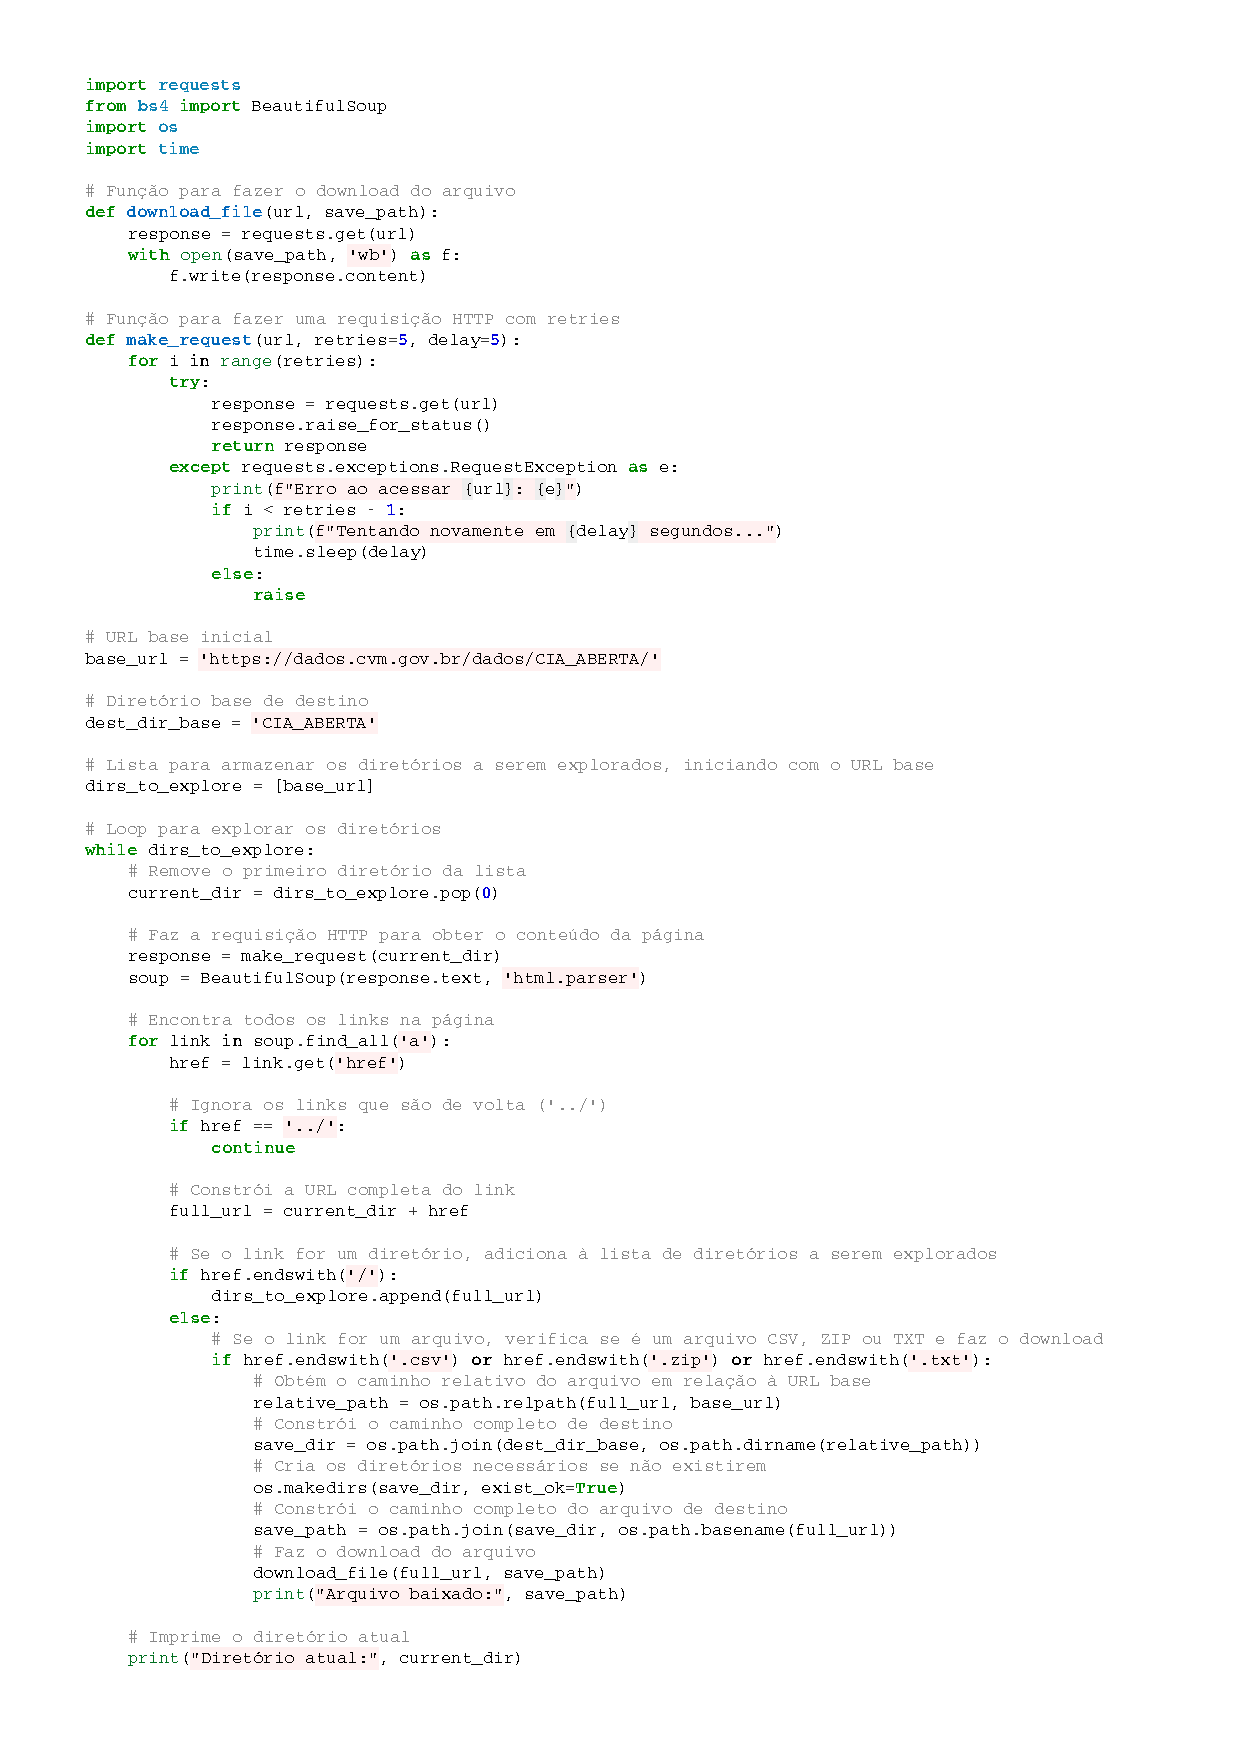
\includepdf[pages=-,frame=true]{codigo/baixar.pdf}

\chapter{Código para extrair os dados da CVM}
\label{ap:codigo-extrair}
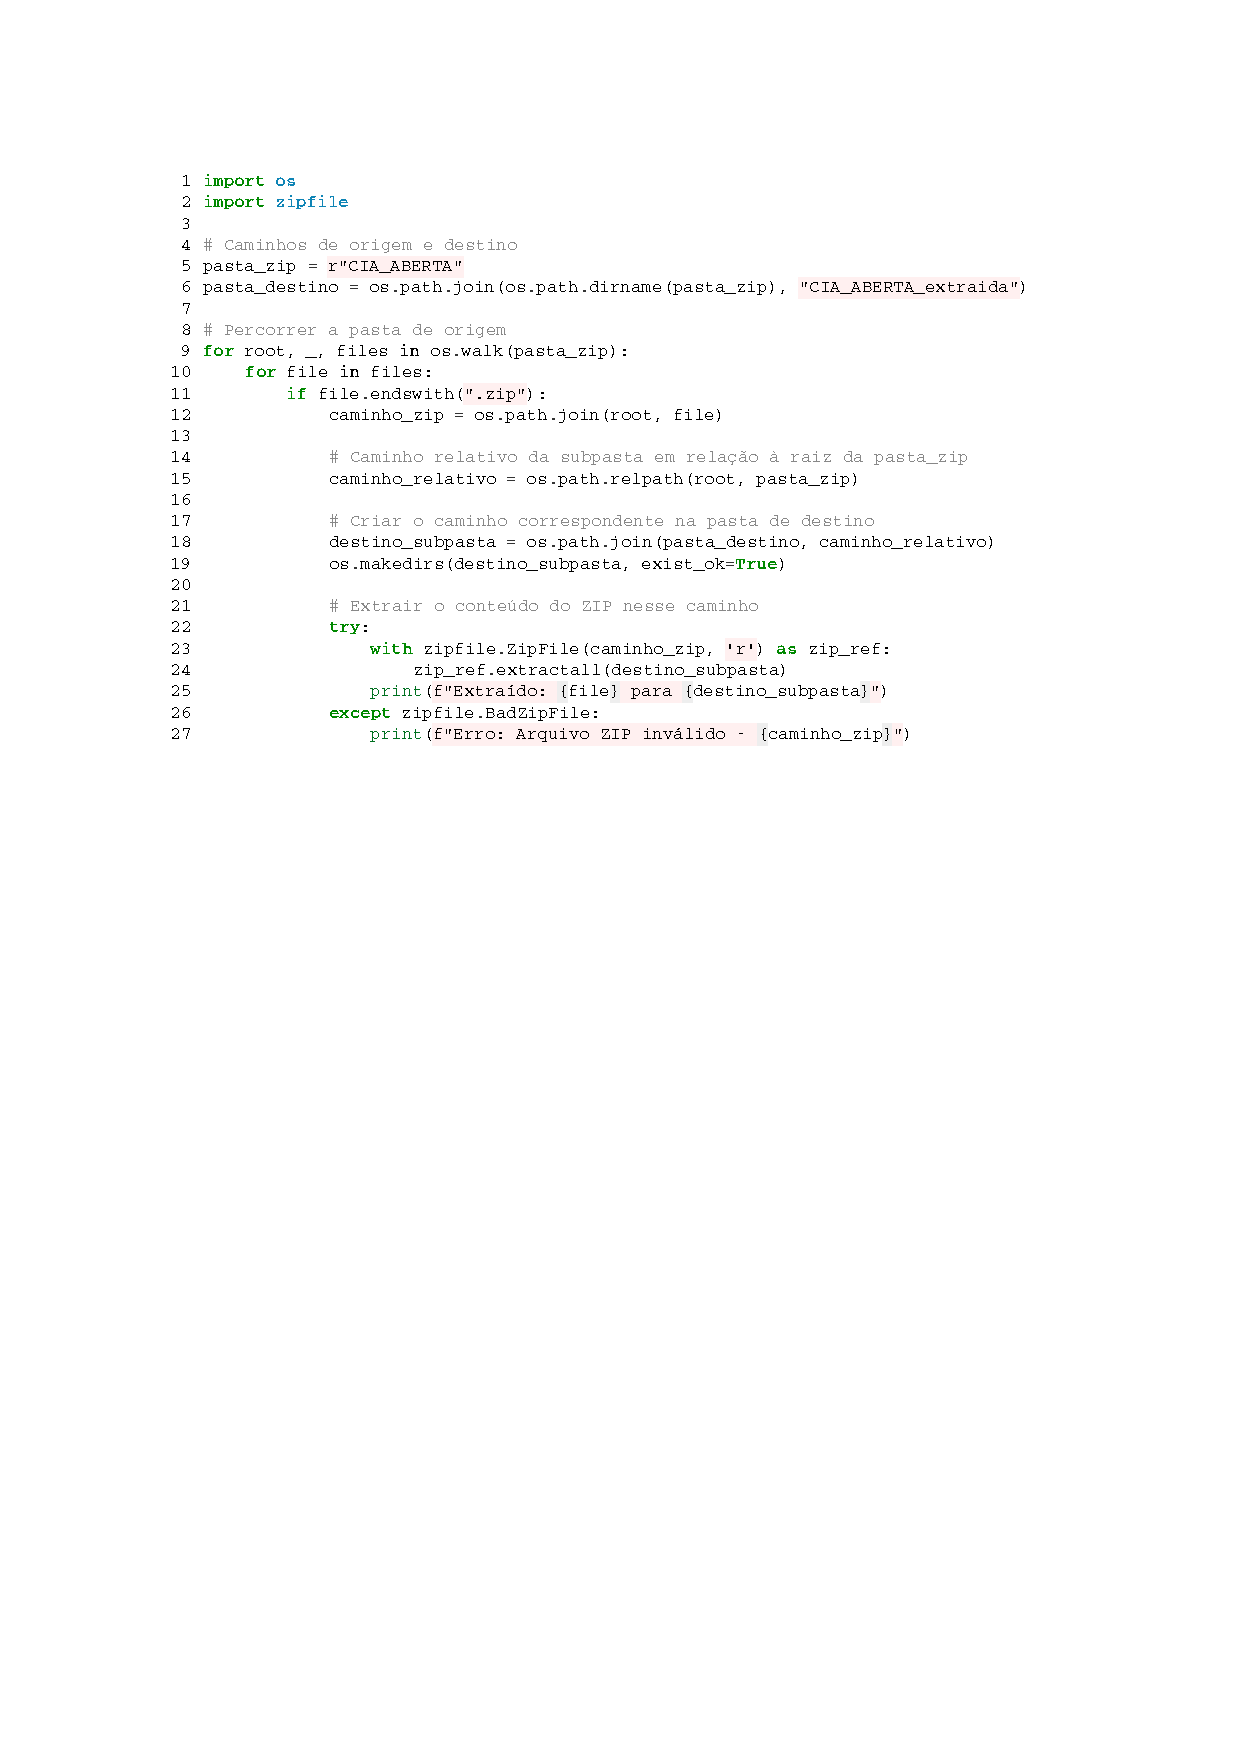
\includepdf[pages=-,frame=true]{codigo/extrair.pdf}

\chapter{Mapeamento Completo dos Dados da CVM}
\label{ap:mapeamento-cvm-dfp}
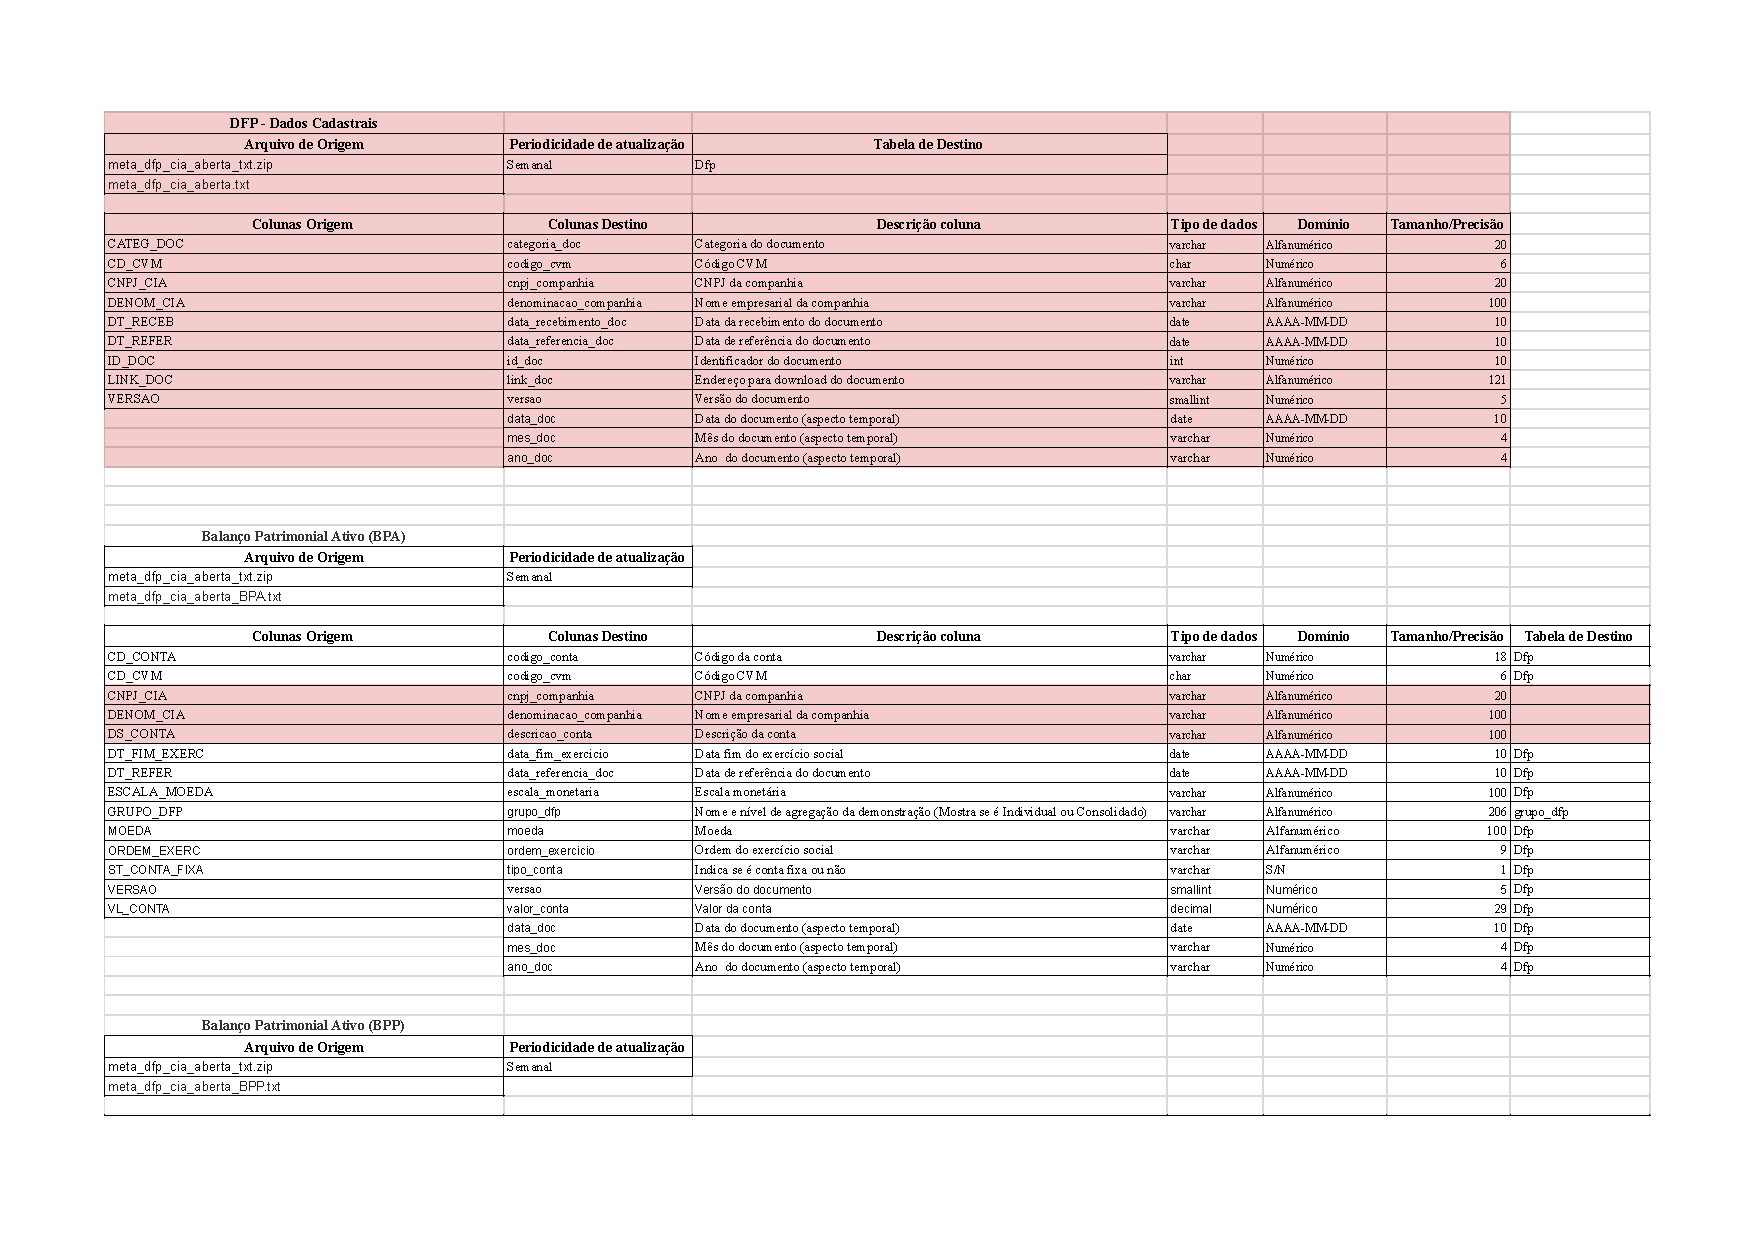
\includepdf[pages=-,frame=true]{apendice/Mapeamento CIA Aberta.pdf}

\chapter{Primeira modelagem}
\label{ap:esquema-inicial}
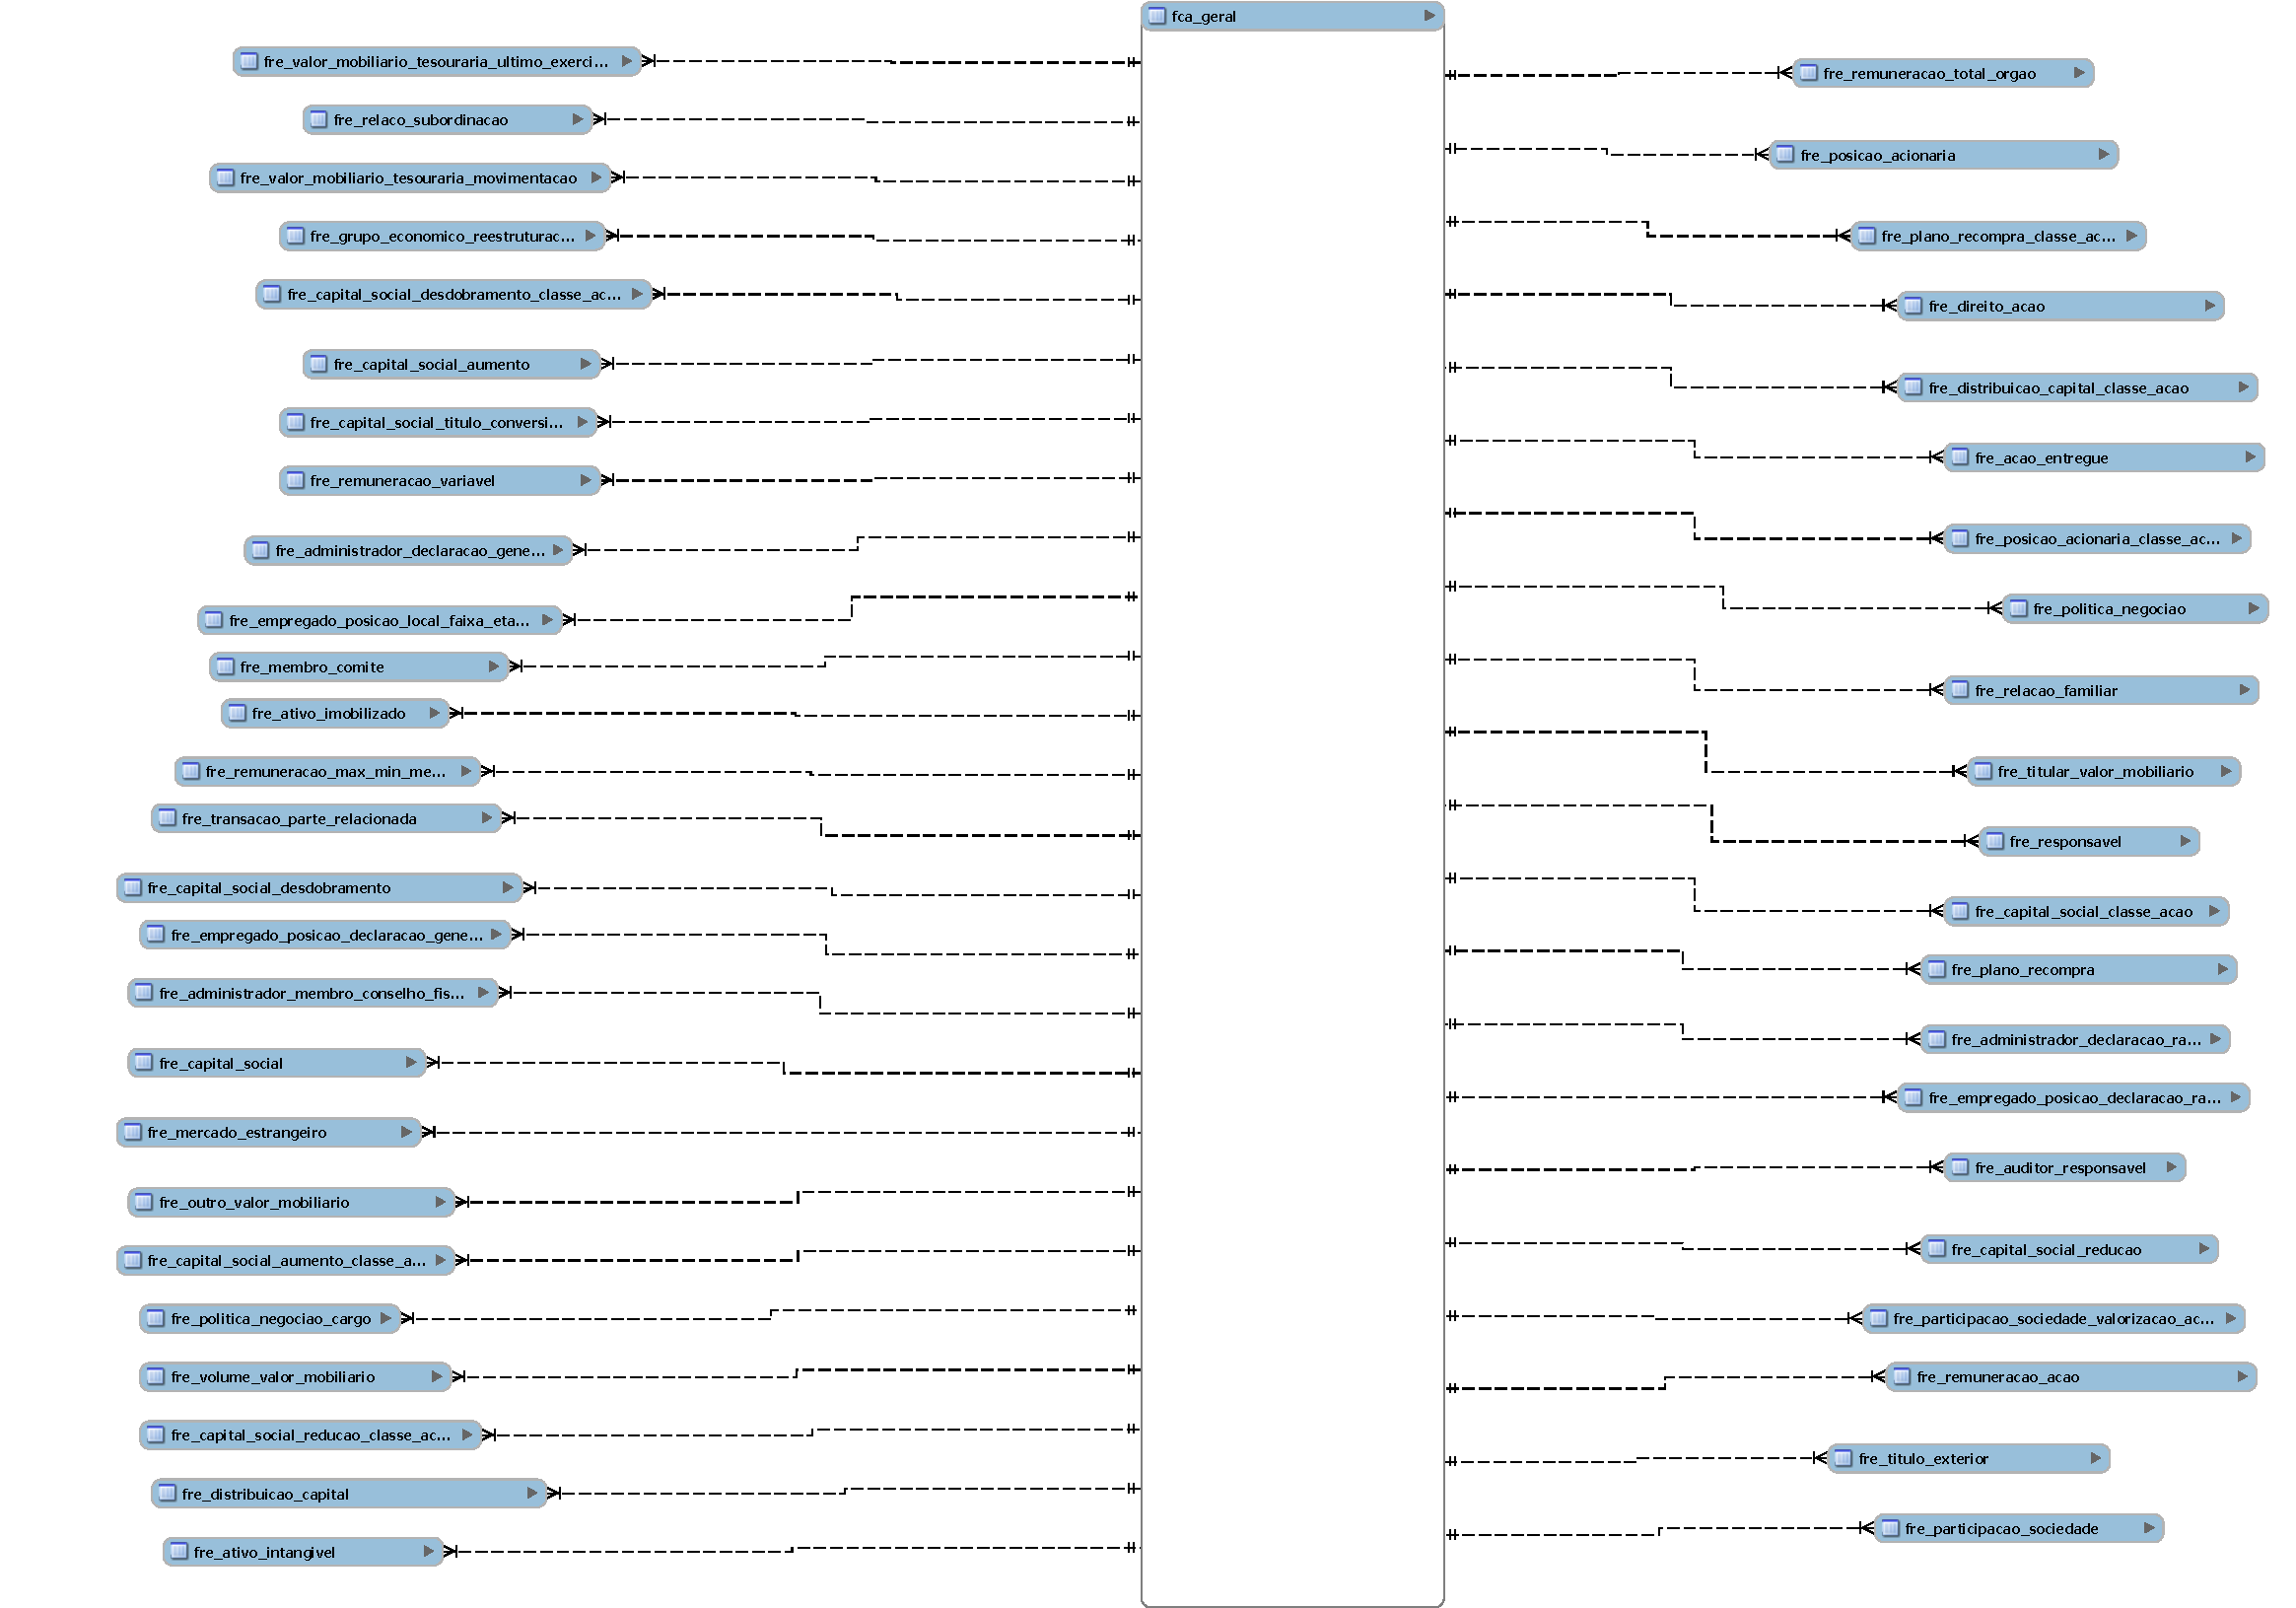
\includepdf[pages=-,frame=true]{apendice/esquema primeira modelagem.pdf}

\chapter{Modelagem apos ajustes iniciais}
\label{ap:esquema-algumas-modelagens}
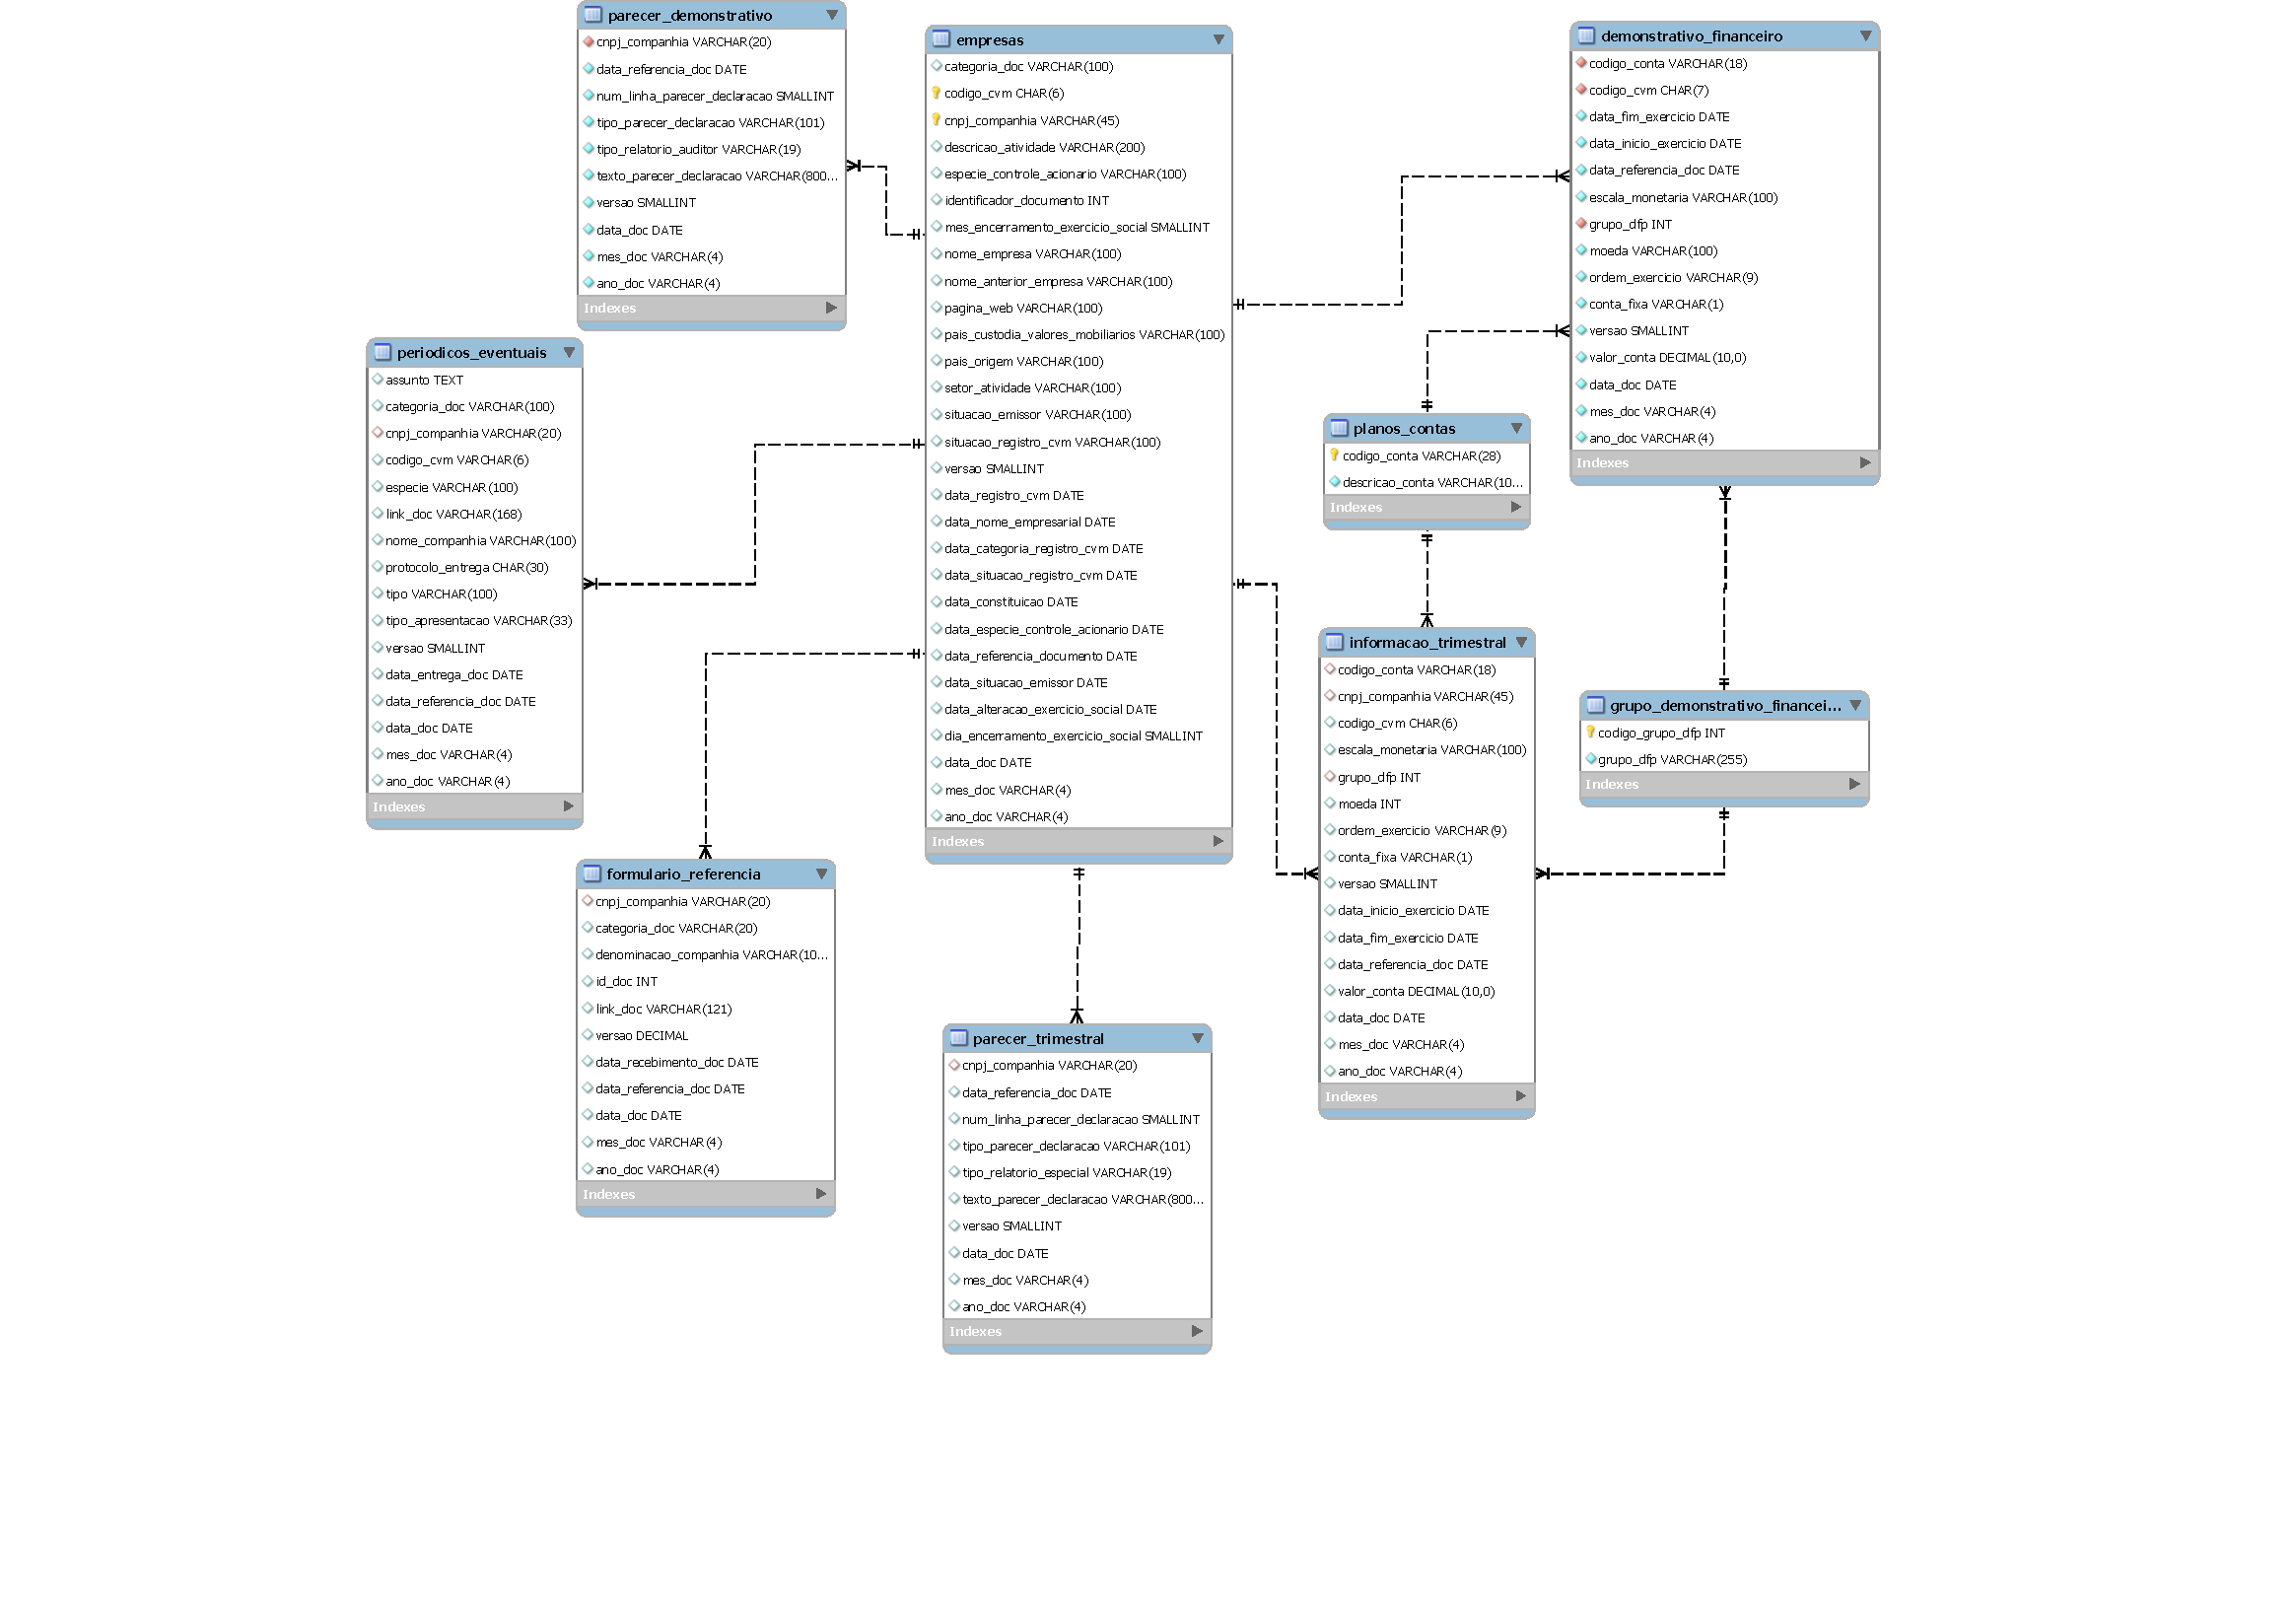
\includepdf[pages=-,frame=true]{apendice/esquema algumas modelagem depois.pdf}

\chapter{Penúltima modelagem}
\label{ap:esquema-penultima-modelagem}
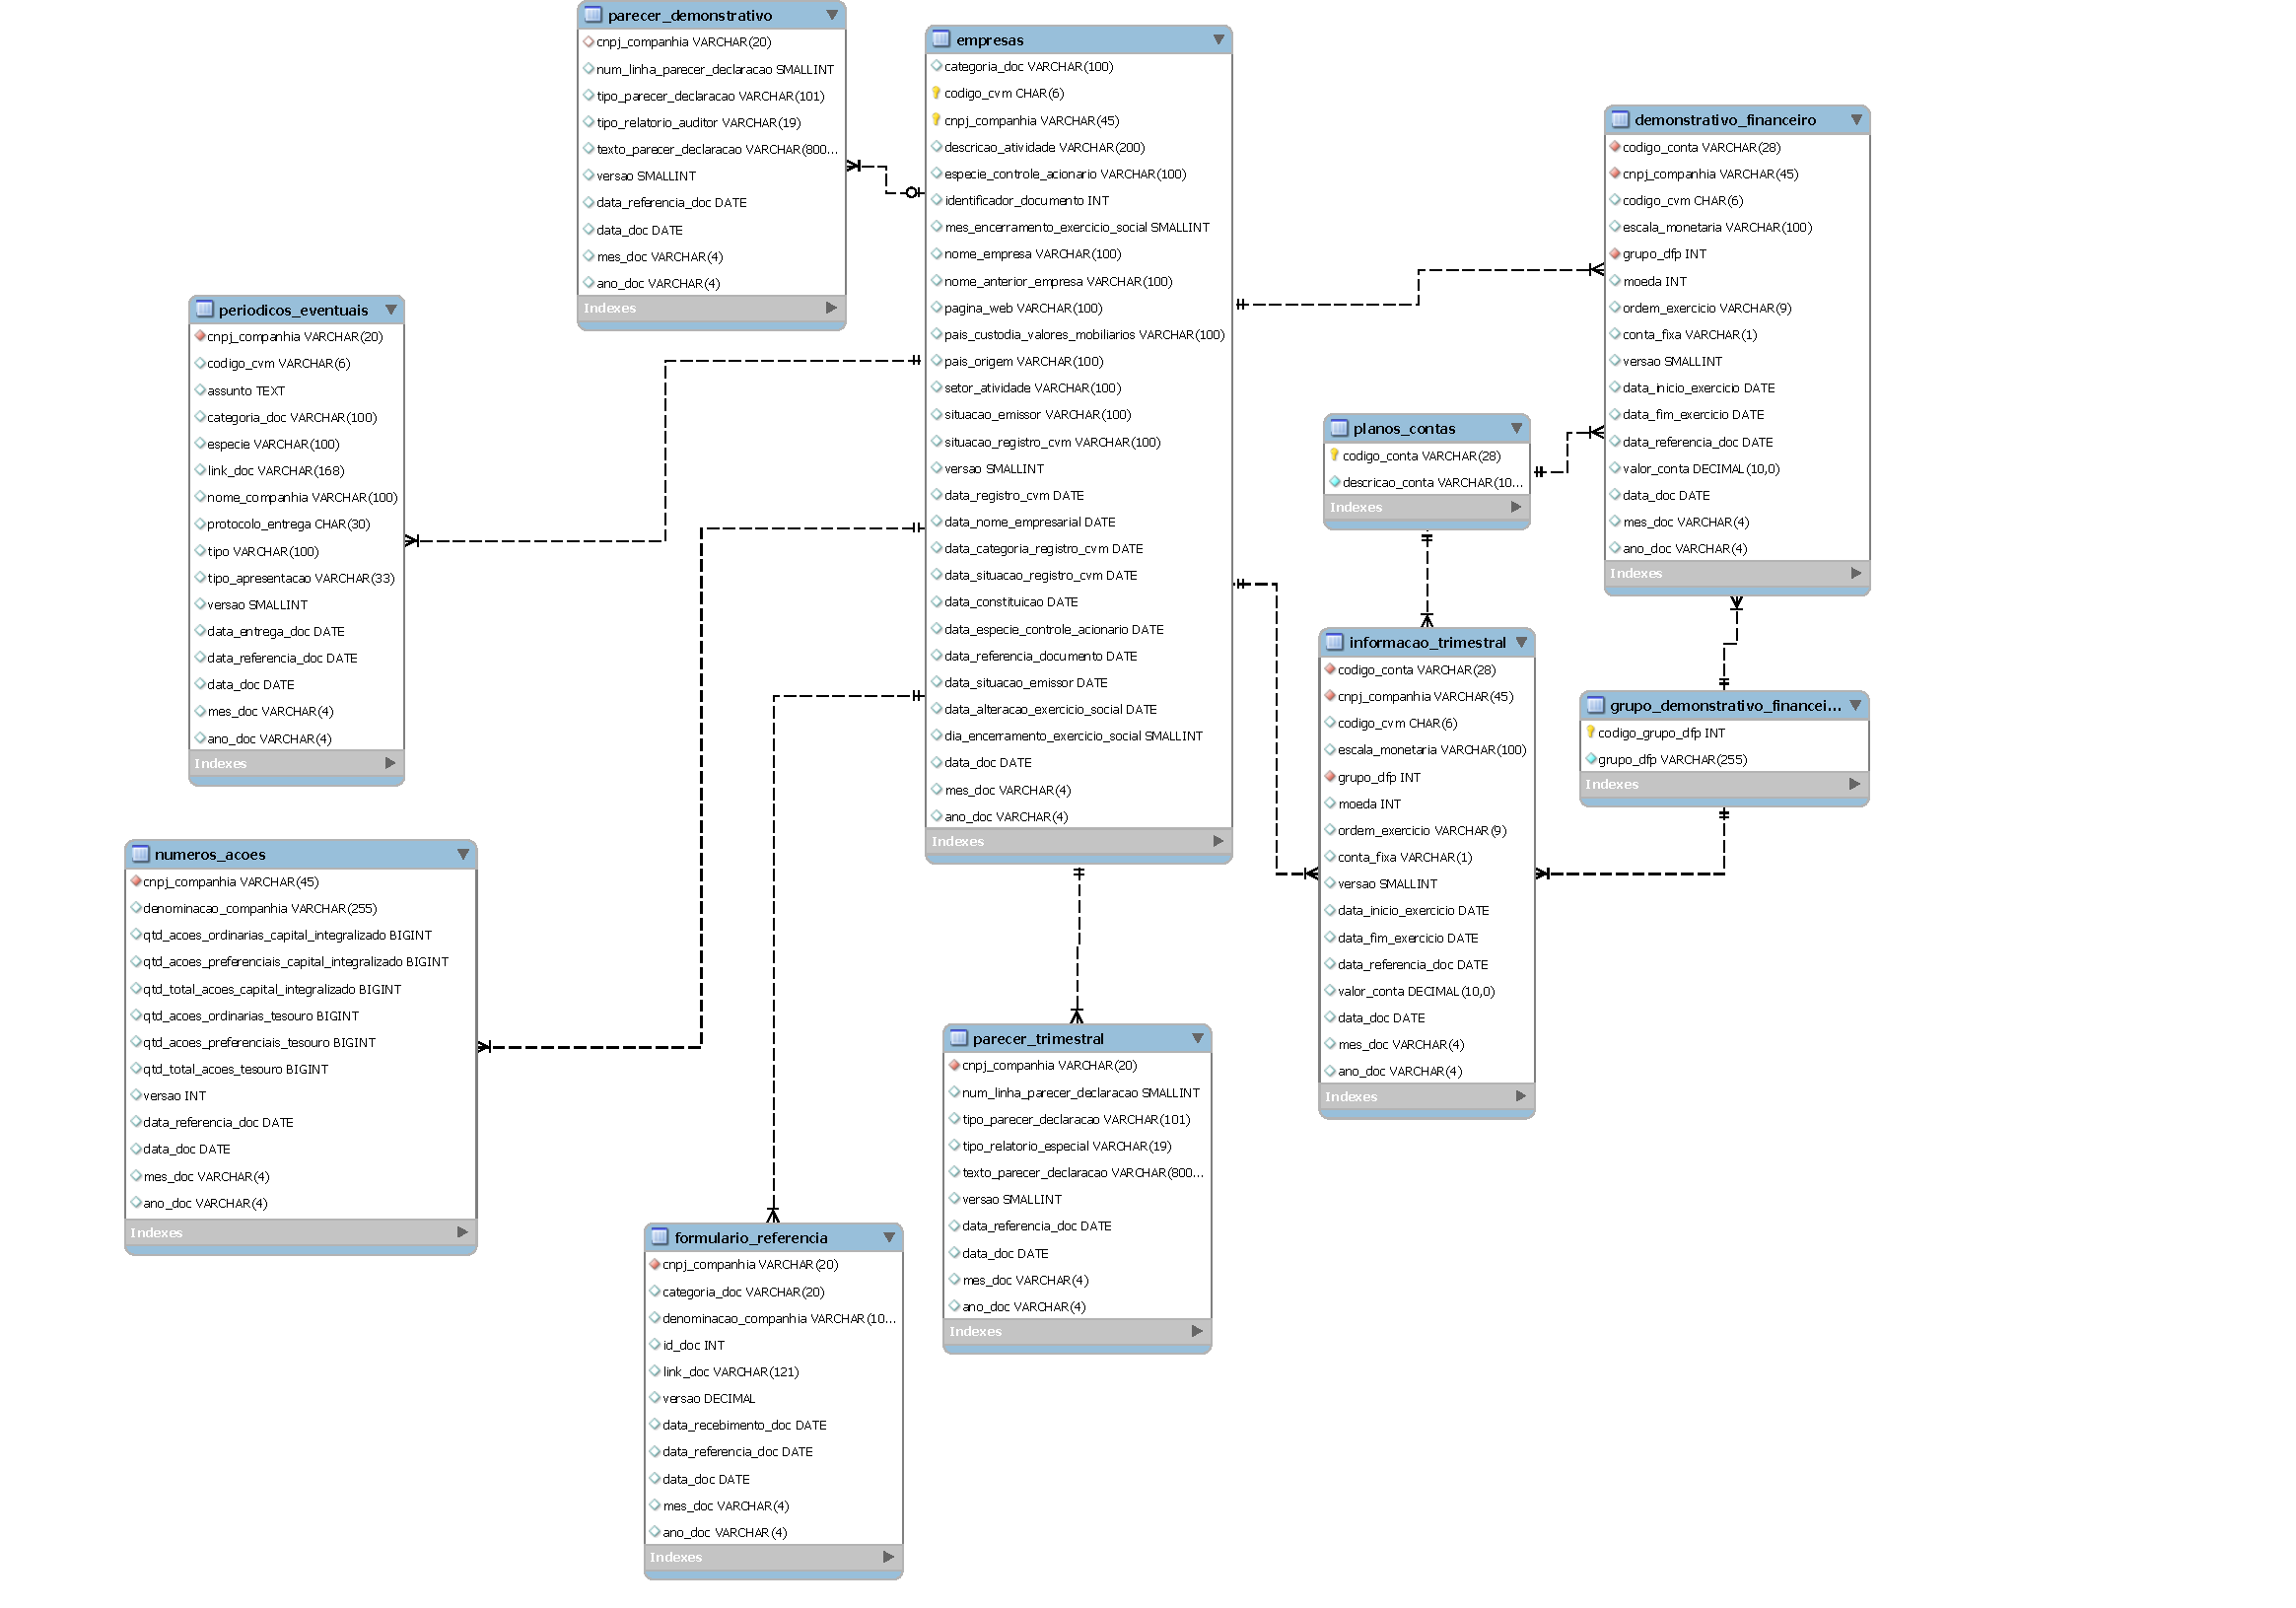
\includepdf[pages=-,frame=true]{apendice/esquema penultima modelagem.pdf}

\chapter{Modelagem presente no código}
\label{ap:esquema-logico-ultimo-presente-no-codigo}
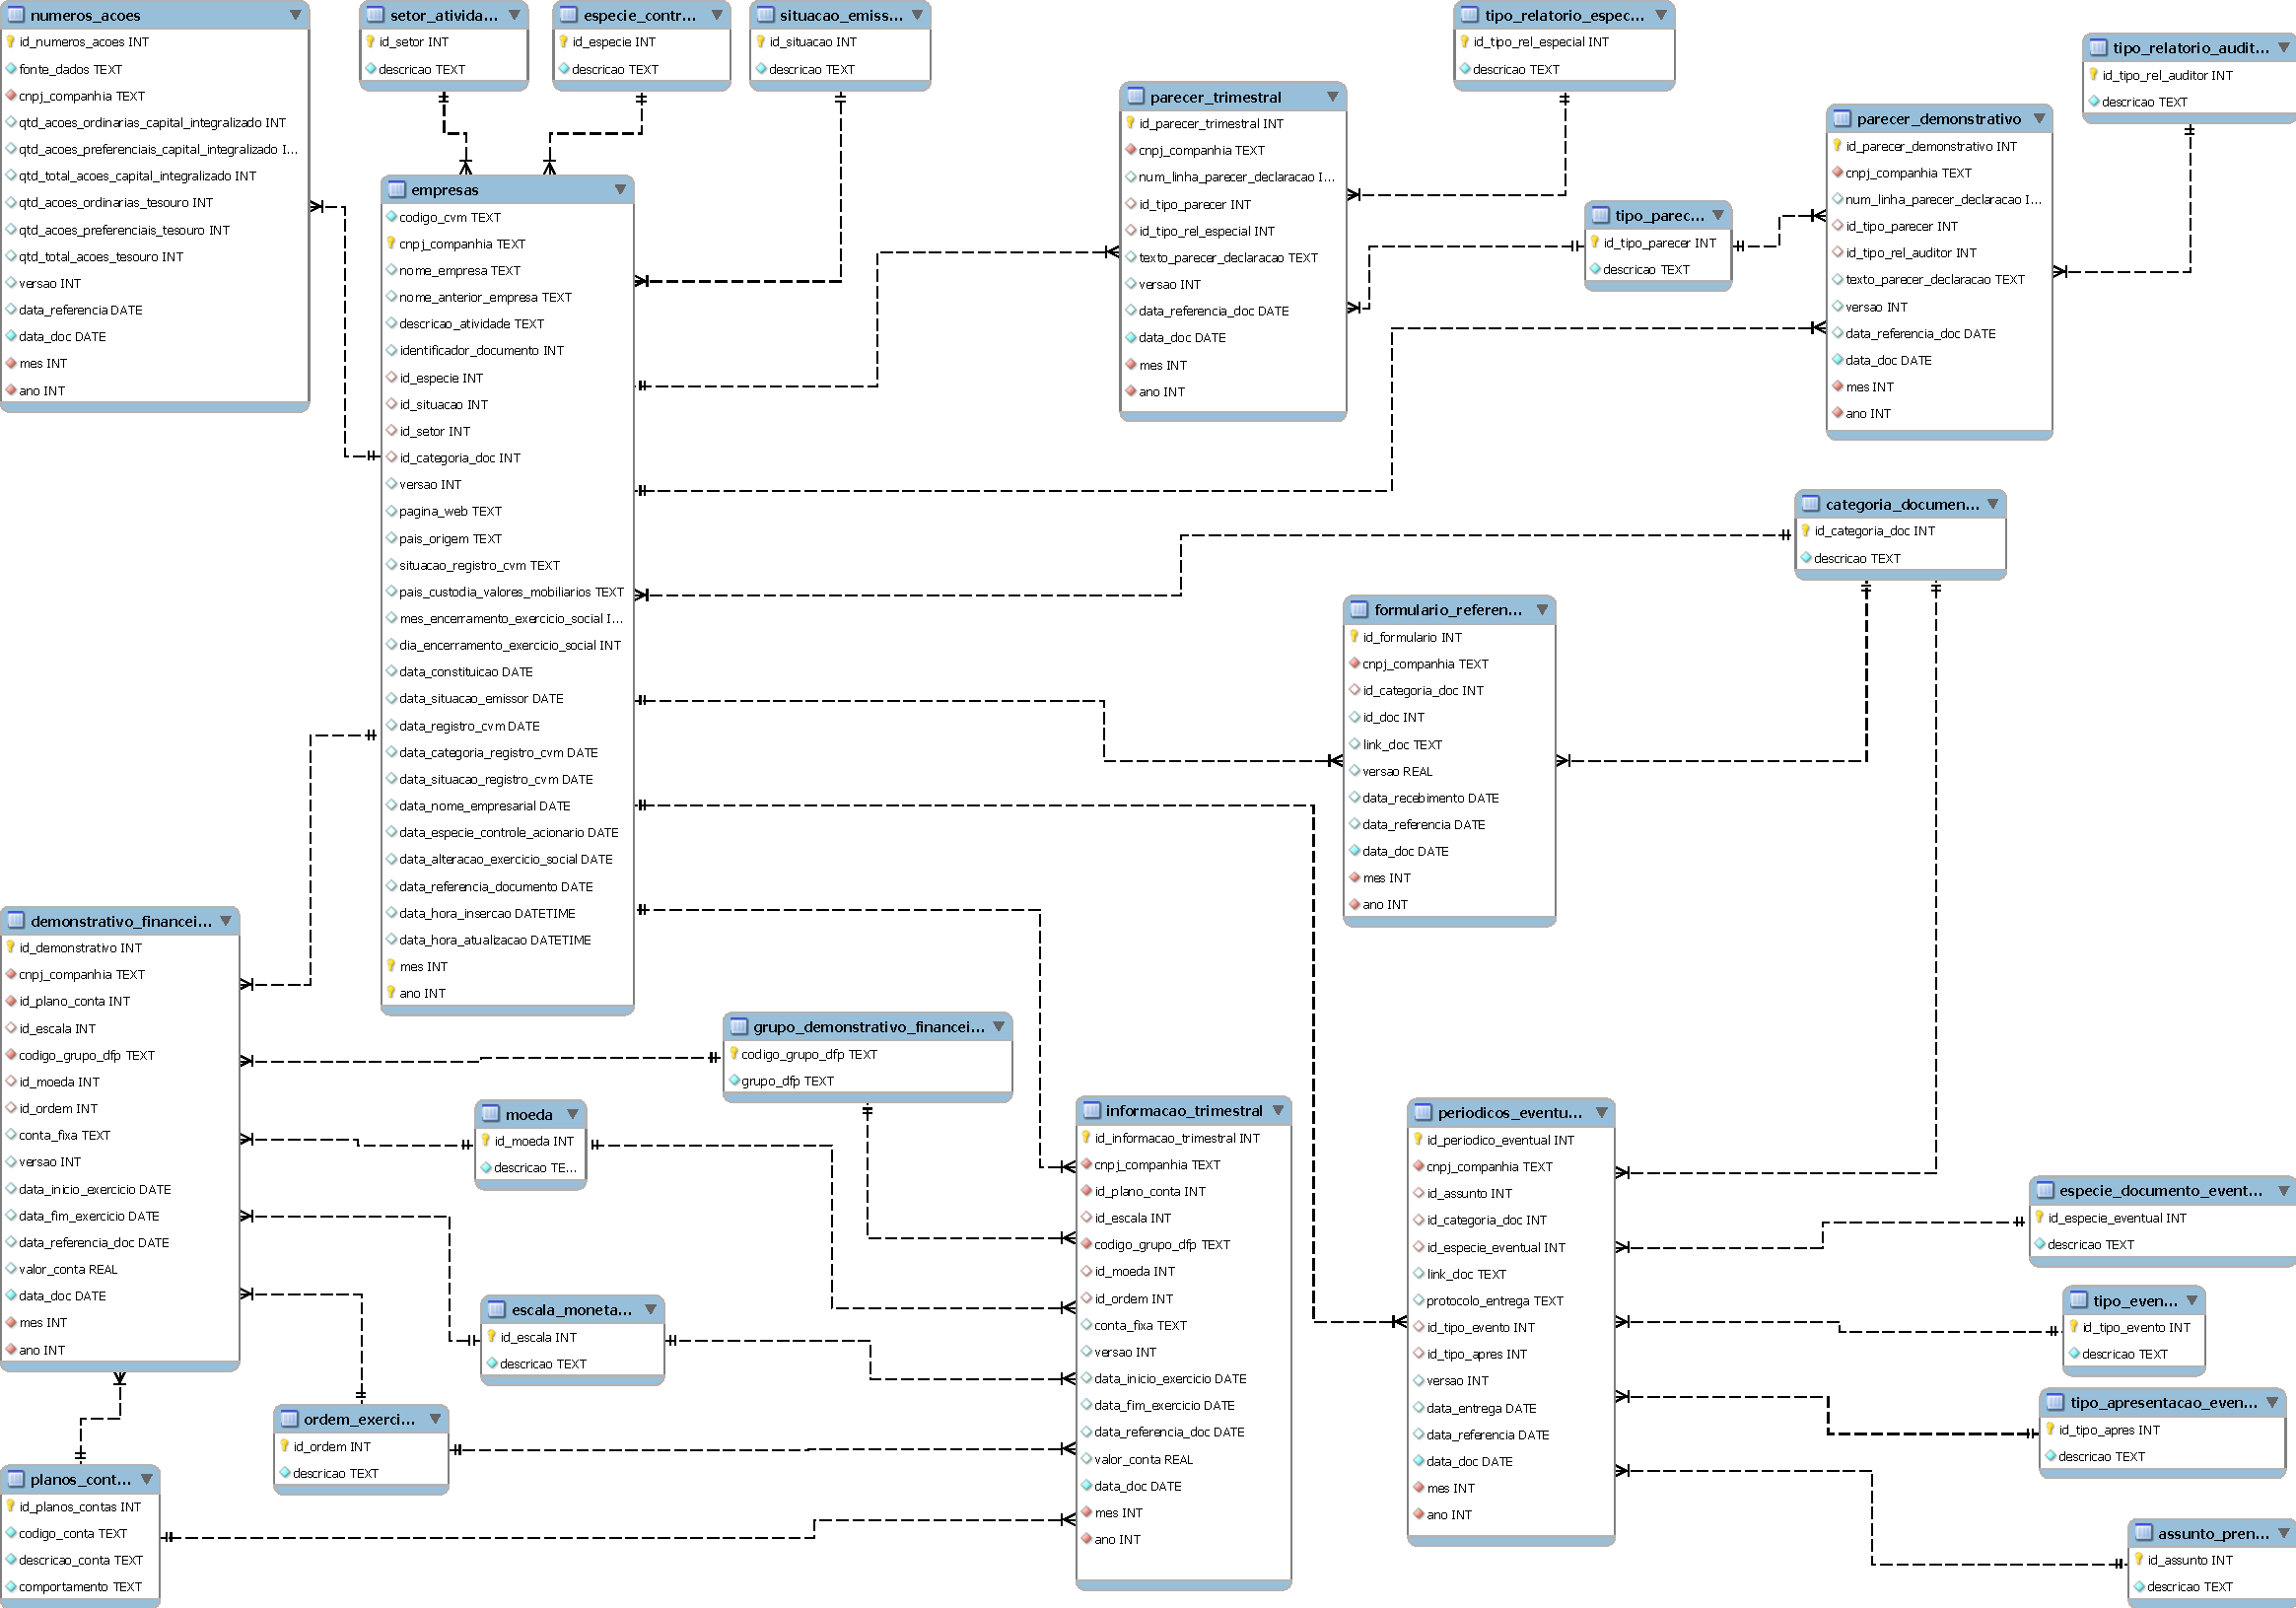
\includepdf[pages=-,frame=true]{apendice/esquema-logico ultimo presente no codgio.pdf}

\chapter*{ÍNDICE}

\printindex

\end{document}
